% https://habr.com/ru/companies/ruvds/articles/574352/
% https://guides.nyu.edu/LaTeX/sample-document
% https://ru.stackoverflow.com/questions/222769/latex-как-быть-с-русским-текстом/757767#757767

\documentclass{article}
% без этой строчки (модуль cmap) не будет работать поиск внутри документа и копирование русского текста:
\usepackage{cmap}
\usepackage[utf8]{inputenc}
% чтобы работал символ евро €
% https://tex.stackexchange.com/questions/9866/latest-advice-on-the-euro-symbol#9868
\usepackage{lmodern,textcomp}
\usepackage[english,russian]{babel}

% разбить длинные адреса URL, которые не умещаются в строку
% https://tex.stackexchange.com/questions/54946/how-to-break-a-long-url
\usepackage[hyphenbreaks]{breakurl}
\usepackage[hyphens]{url}

% слова с дефисом (здесь в основном - "аппаратно-программная") по умолчанию не переносятся автоматом и вылезают за пределы строки
% чтобы этого не происходило, следует заменить дефис на команду "=
% https://www.linux.org.ru/forum/general/11119398
% http://www.inp.nsk.su/~baldin/LaTeX/ctex.pdf
% https://stackoverflow.com/questions/2193307/how-do-i-get-latex-to-hyphenate-a-word-that-contains-a-dash
% в текущем документе работает без подключения дополнительных модулей (в смысле, необходимые модули уже и так подключены выше)
% заменяю только в тех случаях, где после экспорта в pdf строки, действительно, вылезают за границы
% (в консоли вывода pdflatex в этом случае будет предупреждение "Overfull \hbox")

% \raggedright внутри \section - отключить перенос слов внутри заголовка
% https://www.linux.org.ru/forum/general/11676660

\usepackage{graphicx}

\title{Экономические модели распространения цифровых продуктов}
\author{А.~Е.~Моисеев}
\date{сентябрь 2024}
%\date \today

\graphicspath{ {img/} }

\begin{document}

\maketitle

Внедрение технологий, основанных на автоматических цифровых вычислениях, позволяет потребителям повышать производительность труда — создавать больше стоимости на производстве или сокращать непроизводственные издержки, таким образом достигать экономического эффекта \cite{ecoEffects}. Стремление получить экономический эффект — объективный стимул покупки и внедрения технологического продукта. С точки зрения потребителя, результат сравнения цены продукта и потенциального экономического эффекта, который от его внедрения можно ожидать, является объективным критерием принятия решения о покупке. С точки зрения производителя продукта, совокупный экономический эффект, который может быть достигнут всеми потенциальными потребителями продукта на рынке, является верхней границей ресурсов рынка, на которые он может претендовать.

Экономический эффект от внедрения ПО достигается при исполнении программных алгоритмов на аппаратной платформе. Чем больше действующих установок программного продукта развернуто и эксплуатируется по назначению, тем больший суммарный экономический эффект они произведут. Программное обеспечение может распространяться как «чистое» ПО, когда наличие вычислительной техники у потребителя подразумевается как исходная предпосылка распространения программного модуля, или в составе аппаратно-программной платформы. В случае с вариантом аппаратно-программной платформы количество копий программы привязано к количеству произведенных и проданных устройств. В случае с «чистым» ПО возможности распространения программного продукта ограничены распространенностью целевой аппаратной платформы\footnote{«If hardware vendors could increase the number of households with microcomputers, then software developers could sell enough copies of their programs to recoup their initial investment.» \cite{driscollOpenLetter}}.

% команда \chapter недоступна в documentclass article
%\chapter{Аппаратно-программные платформы}
\section*{\raggedright{Аппаратно-программные платформы}}

Аппаратно-программные платформы: бытовая техника с встроенными микроконтроллерами, гаджеты, роботы, станки с ЧПУ и т.~п. Программное обеспечение наделяет аппаратную часть необходимыми потребительными свойствами: микроволновая печь, стиральная машина с цифровым управлением или смартфон не сможет работать без загруженного на него базового пакета ПО. Аппаратная платформа без загруженного базового пакета программного обеспечения — незаконченное устройство, полуфабрикат\footnote{«[Y]our marvelous software has allowed them to sell a computer which, without it, none would have touched.» \cite{driscollOpenLetter}}. Аппаратная платформа с загруженным пакетом программного обеспечения — законченное специализированное устройство. Потребитель покупает законченное устройство, включающее программную прошивку, но не отдельный программный пакет. Экономический эффект в таком случае следует рассчитывать от внедрения готового устройства, а не отдельных программных модулей.

Разработка пакета программного обеспечения, предназначенного специально для аппаратно"=программного устройства, — этап инженерно"=конструкторских работ наряду с такими задачами, как выбор и компоновка аппаратных компонент, разработка электронной схемы печатных плат, проектирование корпуса устройства и т.~п. Развертывание программного обеспечения (обычно уже в форме двоичной прошивки) на аппаратной платформе — акт производства наряду с изготовлением деталей и сборкой устройства. 

Разработка ПО происходит один раз для партии из любого количества устройств до этапа серийного производства, производится инженерами"=программистами, тестерами, прочими членами команды разработки. Развертывание прошивки происходит для каждого экземпляра производимого устройства на этапе серийного производства, производится рабочими производственной линии — операторами специального оборудования, а не программистами.

Стоимость инженерно-конструкторских работ, включая стоимость разработки программного обеспечения, — фиксированная величина, не зависящая от объема партии производства спроектированных устройств. Абсолютная суммарная прибыль от продажи партии произведенных устройств будет тем больше, чем больше произведено устройств. Размер партии, запланированной к производству, должен быть достаточно большим для того, чтобы прибыль от её продажи покрыла фиксированные издержки на инженерное проектирование, в том числе на разработку программного обеспечения (Рис. \ref{fig:model_hard_soft}). В том случае, если запланированная партия не достаточно велика настолько, чтобы расчетная прибыль превысила стоимость разработки, запуск проекта не имеет экономического смысла.

\begin{figure}[ht]
    \centering
    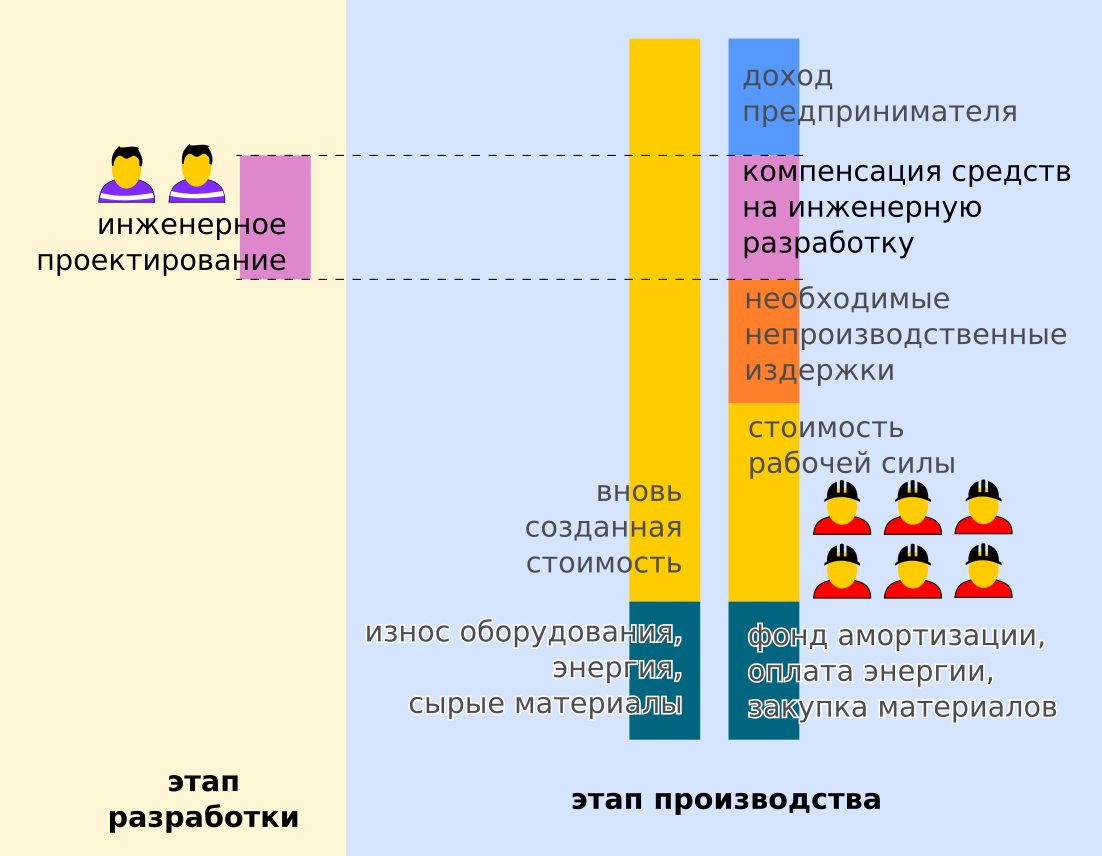
\includegraphics[width=0.6\textwidth]{model-hard-soft}
    \caption{Компенсация расходов на инженерную разработку вычетом из прибыли от произведенной партии спроектированных устройств}
    \label{fig:model_hard_soft}
\end{figure}

В некоторых случаях производитель имеет возможность выпустить обновления для базовой программной прошивки и распространить их через такие механизмы, как OTA (over the air update — обновление «по воздуху») для смартфонов, или бесплатные обновления безопасности на сайте производителя. В таком случае издержки на разработку программного кода обновления переносятся на период, следующий за стадией производства и продажи устройств. Однако и в этом случае стоимость разработки каждого обновления остаётся фиксированной величиной и сама по себе не зависит от количества выпущенных ранее и проданных устройств. Крупнейшие производители смартфонов на платформе Google Android выпускают от двух до семи значительных обновлений системы за срок от двух до семи лет после релиза устройства\footnote{«OnePlus, OPPO, and Xiaomi offer very good update policies, but only for their premium flagships. Mid-rangers and budget models see much weaker promises. Even huge brands like Sony, Motorola, ASUS, realme, and TCL can’t meet the bar set by Samsung’s budget lines.» \cite{phoneUpdates}}, при этом больше внимания уделяют флагманским моделям и меньше — бюджетным.

\section*{\raggedright{Издержки на разработку ПО}}

В современной индустрии разработки программного обеспечения сложно представить проект, который был бы написан силами одной команды абсолютно «с нуля». Так или иначе любая разработка задействует ранее написанный код — стандартную библиотеку языка, драйверы устройств, операционную систему, прочие сторонние библиотеки подпрограмм. Таким образом, любая программная разработка состоит из двух больших частей: новый код, написанный специально для реализации проекта, и старый код, полученный извне, который вызывается из нового кода в виде подпрограмм или работает параллельно с ним на одной аппаратной платформе.

Новый внутренний по отношению к проекту код обычно заточен под конкретный проект и границы его применения очерчены размером партии разработанного устройства. Старый внешний по отношению к проекту код обычно в значительной степени универсален, границы его применимости не очерчены размером партии конкретного устройства — одна и та же программная библиотека применяется в множестве проектов и работает в составе прошивки на множестве разнообразных устройств.

Универсальные программные модули обычно являются разработкой отдельных команд и организаций. Распространяются в форме коммерческого программного обеспечения, например, по модели продажи лицензий, или в форме свободного программного обеспечения — под лицензией, подразумевающей свободное использование, изменение и распространение программного продукта с исходным кодом без обязательных денежных отчислений за право использовать кодовую базу в том числе в коммерческих проектах.

Разработчик коммерческого программного модуля так же, как и непосредственный разработчик устройства, авансирует собственные средства на первоначальную разработку до того, как первая версия модуля войдет в состав прошивки реального устройства. Компенсация средств, потраченных на разработку стороннего программного модуля, в конечном итоге также будет производиться из прибыли от продажи устройств: производитель устройства сначала передаст часть собственных средств разработчику в форме платы за лицензию на программное обеспечение, а потом компенсирует собственные расходы из продажной прибыли. Однако количество применений универсального программного модуля не будет ограничено размером партии конкретного устройства, компенсировать исходную разработку будет не один производитель, а множество игроков (Рис. \ref{fig:model_hard_soft_license_module}). При том, что стоимость исходной разработки модуля остаётся фиксированной, она теперь распределена между большим количеством производителей. Покупка лицензии на программный модуль может обойтись каждому из производителей гораздо дешевле, чем затраты в ситуации, когда бы они разрабатывали аналогичные модули каждый для себя собственными силами.

\begin{figure}[ht]
    \centering
    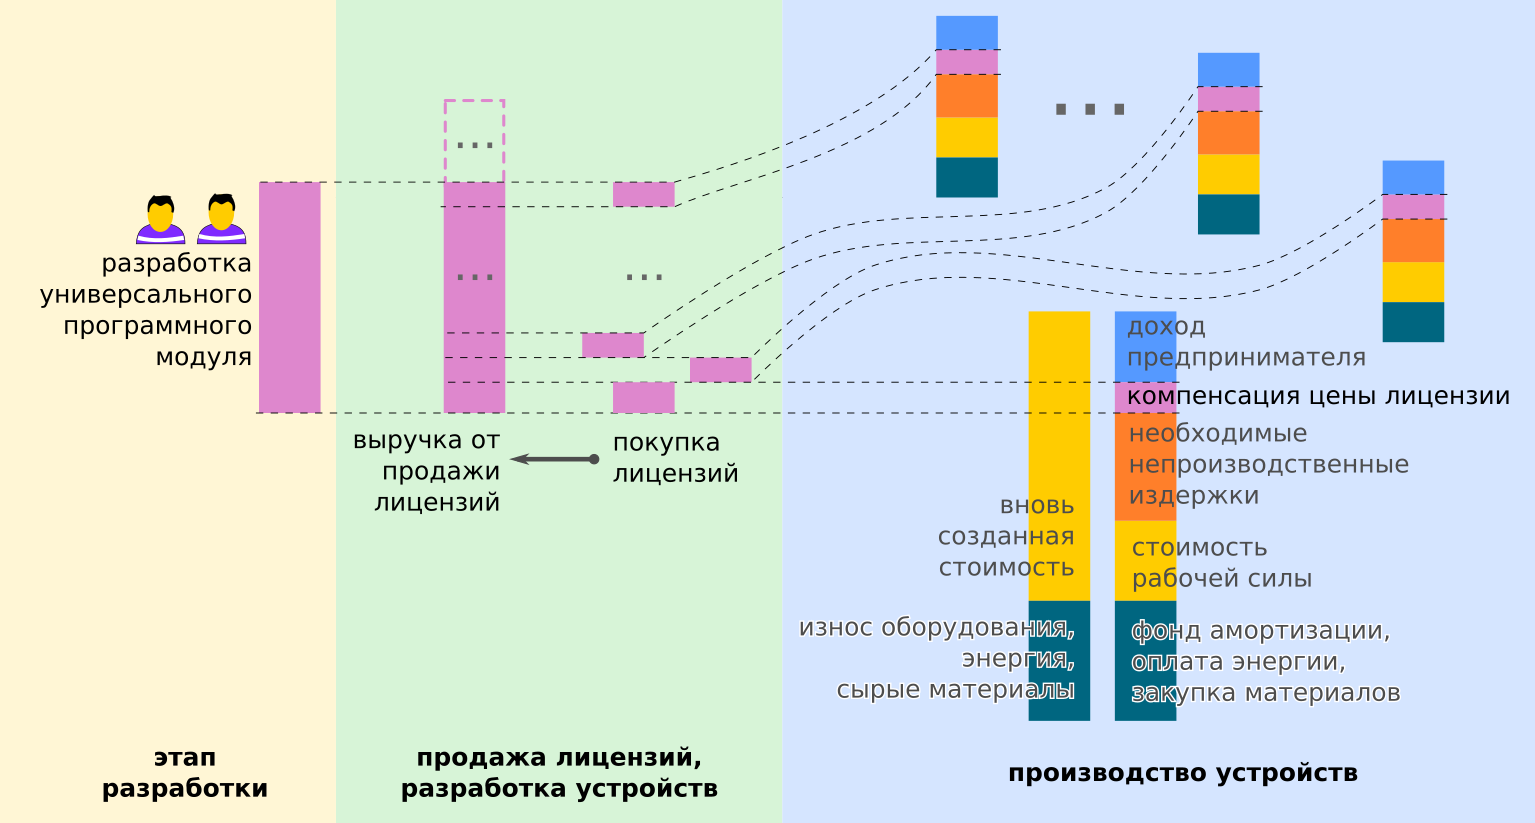
\includegraphics[width=0.95\textwidth]{model-hard-soft-license-module}
    \caption{Компенсация расходов на разработку универсального программного модуля суммой вычетов из прибылей множества производителей, использующих лицензированный модуль}
    \label{fig:model_hard_soft_license_module}
\end{figure}

Для того, чтобы производитель аппаратного обеспечения имел объективный экономический стимул купить лицензию на сторонний коммерческий программный модуль, разработчику программного модуля достаточно выставить такую цену лицензии, которая, во-первых, будет ниже стоимости разработки аналогичного программного модуля силами разработчика аппаратного обеспечения, во-вторых, сможет быть компенсирована разработчиком аппаратного обеспечения из прибыли от продажи целевой партии устройств. Чем большее количество устройств от разных производителей сможет использовать коммерческий программный модуль, тем меньшая цена может быть выставлена на продажу лицензии, тем больше стимула разработчику устройства лицензировать чужой код, а не разрабатывать аналогичный модуль самостоятельно.

Таким образом, наличие сторонних модулей позволяет понизить порог выхода на рынок производителям новых устройств, понижая минимальный размер партии, необходимый для оправдания расходов на разработку программной прошивки.

После того, как все исходные расходы на разработку программного модуля компенсированы из лицензионных отчислений, денежный поток от последующих продаж новых лицензий составит для разработчика коммерческого модуля чистый доход. Он сможет их тратить на поддержку программного продукта (выпуск патчей и обновлений — обычно это незначительные расходы по сравнению со стоимостью исходной разработки), на операционные издержки, а также авансировать на разработку новых проектов (в том числе новых версий существующего продукта), стоимость разработки которых будет компенсирована по такой же модели из будущих применений.

Расходы на разработку свободного программного обеспечения берет на себя общество в целом или отдельные коммерческие игроки, бизнес которых не базируется на модели прямой продажи лицензий на программное обеспечение. Разработчики устройств могут свободно использовать такой код и не платить за него прямых лицензионных отчислений, порог выхода на рынок таким образом для них опускается еще ниже.

Однако любой программный продукт, как коммерческий, так и с открытым исходным кодом, может требовать дополнительный труд по доработке и настройке для задач конкретного проекта. Эти задачи решит внутренняя команда разработчиков проекта, поэтому применение сторонних программных модулей может значительно понизить стоимость разработки программного обеспечения для устройства, но в большинстве случаев не сможет обратить её в ноль.

\section*{\raggedright{Компенсация средств, авансированных на разработку программного обеспечения, из экономических эффектов: бизнес-модели распространения и продажи ПО}}

Создание нового программного продукта занимает продолжительное время, в течение этого времени он не может быть использован по назначению. Издержки на первоначальную разработку покрываются авансом из первоначальных инвестиций — накопленного капитала. На первых этапах (стадия разработки) они значительны, после того, как продукт разработан и стабилизирован (стадия эксплуатации), их можно радикально сократить.

На этапе разработки инженеры"=программисты получают средства инвестора — эти средства составят стоимость разработки. На этапе эксплуатации и продаж инвестор возвращает себе средства, потраченные на инженеров"=разработчиков. Средства, полученные от продаж, компания"=разработчик может реинвестировать\footnote{«A significant investment is made to develop products. And survival is dependent on our partners’ ability to distribute and license products so that a reinvestment can be made into research and development to create new and better software products to meet consumers’ needs.» \cite{microsoftPiracyReinvest}} в создание новой версии программного продукта с тем же названием и той же командой так, что со стороны это будет выглядеть, как непрерывный процесс разработки одного и того же программного продукта. Однако, в действительности, на стадии эксплуатации, приносящей доход, будет находиться продукт старой версии, а продукт новой не выпущенной в эксплуатацию версии будет находиться на стадии разработки, на которой средства расходуются на команду разработки, но не возвращаются до тех пор, пока новая версия продукта не перейдет в стадию эксплуатации.

Объективный стимул внедрения программного продукта его потребителем — желание получить новую добавочную стоимость (или необходимость тратить не больше, чем остальные), т.~е. реализовать экономический эффект. Часть этой новой или высвободившейся стоимости — источник средств, из которых потребитель сможет сначала компенсировать собственные расходы на покупку и внедрение программного продукта, которые, в свою очередь, ранее уже компенсировали разработчику средства, потраченные на разработку программного продукта. Т.~е., в конечном итоге, первоначальные расходы, направленные инвестором на разработку программного продукта, будут компенсированы частью суммарного экономического эффекта от внедрений этого программного продукта среди всех его потребителей во всём обществе.

Теперь задача разработчика — организовать канал движения средств, через который он эту стоимость сможет получить от внедряющей программный продукт стороны. Вопросы на этом этапе — целевая бизнес-модель и ценообразование.

\section*{\raggedright{Внутрикорпоративная разработка}}

Результат разработки внедряется и используется исключительно внутри компании, не используется за её пределами. Источник финансирования — свободные собственные средства компании — накопленный капитал. Разработка может быть проведена внутренним отделом ИТ или заказана на стороне с условием передачи исключительных прав на использование продукта внутри компании-заказчика. Экономический эффект от внедрения разработанного продукта окупит первоначальные издержки на разработку (Рис. \ref{fig:model_eco_effect_corporate}), далее компания продолжит работу с новой повышенной производительностью труда. Компания должна быть достаточно крупной для того, чтобы общий экономический эффект от внедрения разработанного программного пакета окупил издержки на его разработку. Чем больше компания, тем больший масштаб внутренних разработок она может себе позволить.

\begin{figure}[ht]
    \centering
    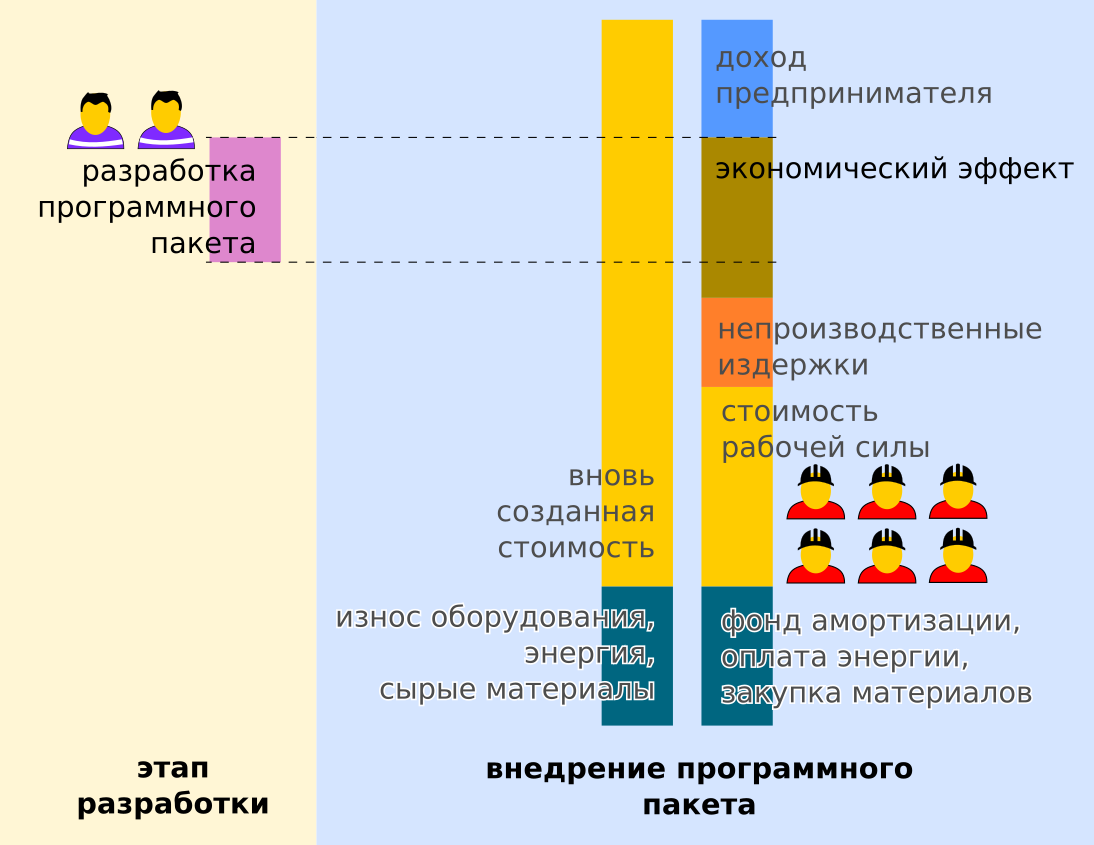
\includegraphics[width=0.6\textwidth]{model-eco-effect-corporate}
    \caption{Компенсация расходов на разработку внутрикорпотаривного программного пакета реализацией экономического эффекта внедрения пакета внутри предприятия}
    \label{fig:model_eco_effect_corporate}
\end{figure}

Некоторые платформы автоматизации бизнеса такие, как 1С, позволяют создавать персонализированные продукты, при этом возможности базовой платформы снижают стоимость разработки индивидуальных конфигураций. Базовая платформа выступает полуфабрикатом, в производственный процесс внедряется построенная на его базе индивидуальная конфигурация. Стоимость разработки индивидуальной конфигурации компенсируется при этом целиком из экономического эффекта единственного потребителя, стоимость разработки базовой платформы компенсируется по модели коммерциализации тиражируемого массово программного продукта.

В некоторых случаях корпорации превращают свои внутренние разработки в продукты, доступные для широкого круга потребителей, — публикуют их как свободное программное обеспечение\footnote{«Though Facebook has all but abandoned Cassandra, the technology has gone on to power critical web infrastructure at companies like Twitter, Netflix, even Apple. <...> According to data compiled by Austrian consulting firm Solid IT, Cassandra is the second most popular NoSQL database in the world» \cite{facebookCassandra}}\footnote{«Яндекс опубликовал исходный код распределённой системы управления базами данных YDB. <...> Надёжность YDB проверена на масштабах Яндекса, где она используется больше 5 лет. Проекты в YDB размещают команды Алисы, Такси, Маркета, Метрики и других сервисов — сейчас в системе почти 500 проектов.» \cite{yandexYDB}}\footnote{«Изначально СУБД ClickHouse была разработана в «Яндексе» для обработки логов «Яндекс.метрики». <...> В июне 2016 г. «Яндекс» выложил технологию в открытый доступ <...> Сейчас открытым кодом ClickHouse пользуются в сотнях компаний, включая Uber, Tesla, Spotify, eBay, ByteDance, Alibaba, Tencent.» \cite{yandexClickHouse}}\footnote{«It's not selling access to its deep learning engine. It's open sourcing that engine, freely sharing the underlying code with the world at large. This software is called TensorFlow, and in literally giving the technology away, Google believes it can accelerate the evolution of AI.» \cite{googleTensorFlow}} или как коммерческое программное обеспечение\footnote{«Корпоративные наукоёмкие программные продукты позволяют нам решать сложные инженерные задачи быстрее, экономичнее и с меньшими рисками. Программное обеспечение используют в своей работе все дочерние предприятия “Роснефти”. Более 1200 лицензий реализовано крупным промышленным компаниям нефтегазовой отрасли.» \cite{rosneftSoft}}. Реализация экономического эффекта в таком случае выходит за границы компании, издержки на разработку остаются прежними\footnote{«Эту инициативу глава Минцифры объяснил концентрацией финансовых ресурсов, которые было бы эффективнее направлять на разработку конкурентных продуктов, которыми будет пользоваться весь рынок, а не одна госкомпания-разработчик.» \cite{mintcifriForbidInhouseSoft}}. В том случае, если программный продукт распространяется на коммерческой основе, компания-разработчик получает дополнительный канал прямой компенсации издержек его разработки.

\section*{\raggedright{«Продажа» лицензий и подписка}}

Хотя в документах учёта продажа и покупка лицензионного ПО проводится по особым процедурам\footnote{Международный стандарт финансовой отчетности: «Если программное обеспечение не является неотъемлемой частью оборудования, к которому оно относится, то оно учитывается как нематериальный актив.» \cite{accountingIAS}}\footnote{НК РФ: «К нематериальным активам, в частности, относятся: <...> исключительное право автора и иного правообладателя на использование программы для ЭВМ, базы данных» \cite{accountingNKRF257}}\footnote{НК РФ: «К прочим расходам, связанным с производством и реализацией, относятся следующие расходы налогоплательщика: <...> расходы, связанные с приобретением права на использование программ для ЭВМ и баз данных по договорам с правообладателем (по лицензионным и сублицензионным соглашениям).» \cite{accountingNKRF264}}, к форме сделки лицензирования, т.~е. получения неисключительного права на внедрение и использование программного продукта, часто применяют метафору купли-продажи материального объекта, по крайней мере проводят между процедурами «покупки» лицензии на программный продукт и покупки материального продукта параллели\footnote{«Later, in the historiography of the early 1980s, the open letter offered a useful metonym for the perceived clash of cultures between those who imagined a new economy for software and those who treated computer programs like any other commercial product to be bought and sold.» \cite{driscollOpenLetter}}. Механизм покупки лицензии на ПО даёт возможность разработчику ПО получить компенсацию от потребителя ПО в форме платежа по договору. Таким образом, продав известное количество лицензий, разработчик компенсирует первоначальные издержки на разработку — компенсирует инвестиции, все последующие продажи — чистый доход. Покупатель, получив право и возможность запускать ПО на своём аппаратном обеспечении, внедряет его в процесс производства, повышает производительность труда, компенсирует издержки на покупку лицензии из экономического эффекта автоматизации — сокращения издержек или наращивания производства дополнительного продукта, которые он получил следствием внедрения ПО.

Модель продажи лицензий на первый взгляд интуитивно понятна за счет метафорической аналогии с материальными товарами. Однако природа ПО как интеллектуального продукта определяет стратегию присутствия на рынке и ценообразования ИТ-компаний, отличную от стратегии производителей материальных благ. Цена единицы материального товара определяется издержками на его производство и транспортировку с поправкой на колебания цен под действием спроса и предложения и прочих экономических факторов, производство каждой новой партии одного и того же продукта требует понести известное количество затрат, процесс воспроизводства материальных продуктов цикличен. Стоимость разработки программного продукта конечна, программный продукт не воспроизводится заново для каждого нового внедрения, а создаётся один раз, стоимость создания каждой новой копии программного продута пренебрежимо мала\footnote{«A key characteristic of digital goods is that they have zero marginal cost. Digital goods can be reproduced with no additional cost. Let us estimate the cost of producing one additional copy of an app. <...> These costs are tiny so that, for all practical purposes, the cost of installing one additional copy of the app is zero.» \cite{introToDigital}}. Для того, чтобы рассчитать возможную цену лицензии на копию программного продукта, следует принять во внимание интерес разработчика, с одной стороны, и интерес потребителя — с другой.

Со стороны потребителя максимальная цена, которую целесообразно платить за копию ПО, определяется потенциальным экономическим эффектом от его внедрения. Если цена лицензии на копию ПО окажется выше сэкономленных в результате его внедрения средств, то такая покупка принесет итоговый убыток. Если цена лицензии окажется равной экономическому эффекту, покупатель ничего не выиграет, но и не проиграет от покупки такого ПО. Если цена лицензии окажется ниже экономического эффекта автоматизации, покупатель окажется в плюсе от покупки и внедрения ПО, и это будет являться для него объективным экономическим стимулом совершить покупку.

Т.~к. стоимость создания каждой новой копии программного продукта для разработчика пренебрежимо мала, он может позволить себе выставить любой вариант цены единичной лицензии. Разработчик, тем не менее, ограничен издержками на первоначальную разработку программного продукта, а также некоторым количеством фиксированных (не зависящих от количества «производимых» копий) регулярных операционных издержек. Все проданные лицензии в сумме должны, как минимум, компенсировать эти расходы (Рис. \ref{fig:model_eco_effect_license}). Цена одной лицензии может быть рассчитана как общие издержки на разработку ПО, делёные на количество лицензий, которые можно потенциально продать на выбранном сегменте рынка в оговоренный период.

\begin{figure}[ht]
    \centering
    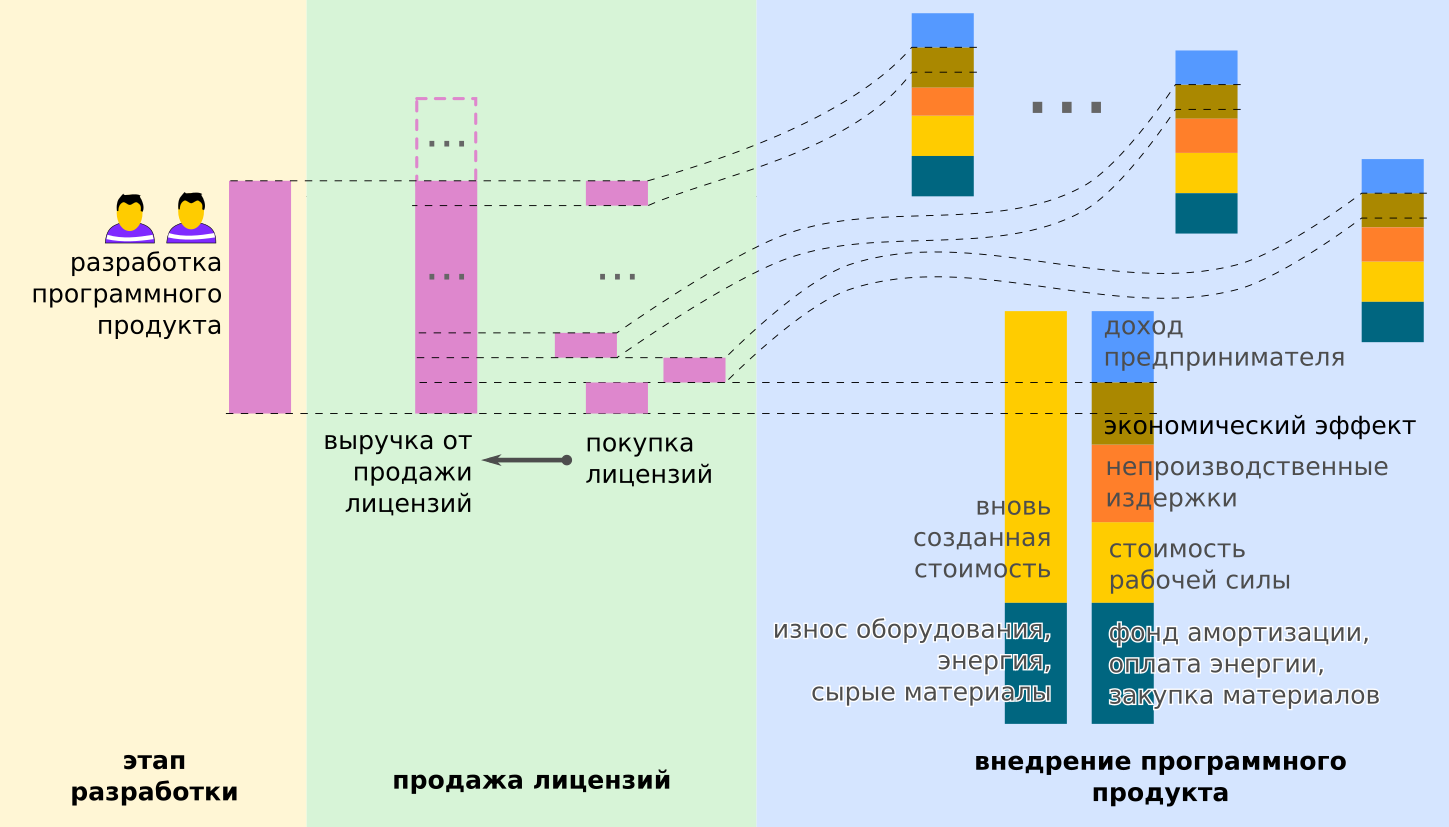
\includegraphics[width=0.95\textwidth]{model-eco-effect-license}
    \caption{Компенсация расходов на разработку лицензируемого программного продукта суммой долей экономических эффектов, реализованных внедрившими продукт потребителями}
    \label{fig:model_eco_effect_license}
\end{figure}

Если рассчитанная по такой формуле цена окажется выше, чем средний ожидаемый экономический эффект автоматизации для большинства потенциальных потребителей ПО, то необходимое количество лицензий не будет продано, разработка изначально не будет иметь шансов окупиться. Если ниже, то разработка проекта имеет смысл.

Покупатели программного продукта — организации или физические лица. После того, как значительная часть всех пользователей купила лицензию и установила ПО, новых продаж не будет. Нужно повторять цикл — выпускать новую версию ПО и продавать новые лицензии\footnote{«While there are plenty of home users still running XP, Microsoft’s big concern is the large number of businesses that haven’t yet upgraded to Windows 7.» \cite{windowsXPLegacy}}. В отличие от материального продукта, программное обеспечение со временем не изнашивается, но оно может морально устареть в том случае, если на рынке появится программный продукт, экономический эффект от внедрения которого в достаточной степени превзойдет экономический эффект от эксплуатации рассматриваемого пакета. Для того, чтобы существующие пользователи программного продукта имели объективный стимул купить его новую версию, экономический эффект от её внедрения должен превышать издержки перехода с предыдущей версии. Таким образом, чтобы обеспечить необходимое количество продаж среди старой базы потребителей, новую версию следует выпускать с достаточным количеством изменений. Или ограничить время жизни лицензии: вместо разовой «покупки» получить регулярные платежи за один и тот же продукт — использовать модель подписки\footnote{«For most of our desktop products on subscription, you don't need to be online to use your software. The software runs on your computer, not on the web. An internet connection is needed initially to install and activate your product.» \cite{autodeskSubscription}}.

При нулевой стоимости копирования продукта компании-разработчики ПО имеют возможность вести гибкую ценовую политику — выставлять разные цены на один и тот же продукт для различных категорий потребителей, в т.~ч. устанавливать нулевые цены в отдельных сегментах, насыщать новый рынок своим ПО с нулевыми затратами (все затраты на разработку уже понесены), вытесняя конкурентов. К примеру, в 2009 году компания Microsoft объявила, что планирует «инвестировать» в Россию 10 млрд. руб. \cite{microsoftInvestsRF}. В действительности в рамках программы планировалось реализовать такие мероприятия, как «запуск в России программы обучения базовым компьютерным навыкам», а также предоставить «более 1000 российских компаний» бесплатно «широкий набор программных продуктов Microsoft», студентам и школьникам — «бесплатный доступ к современным инструментам разработки и дизайна Microsoft». Таким образом, под значительной долей объявленных инвестиций в этом случае подразумевалось не выделение новых средств в денежной форме или форме аппаратного обеспечения, а развертывание новых легальных или легализация существующих установок ПО Microsoft, которые позволили укрепить позиции компании на рынке и были использованы в рекламной кампании, не принеся при этом никаких дополнительных расходов.

\section*{\raggedright{SaaS: «ПО как сервис»}}

Модель SaaS — «Software as a service», «ПО как сервис», «ПО как услуга» подразумевает схему работы с программным обеспечением, запущенным на аппаратном обеспечении продавца сервиса (в т.~н. «облаке»\footnote{Rob Joyce, former chief of the Tailored Access Operations at the U.S. National Security Agency (NSA): «cloud computing is really just a fancy name for someone else’s computer.» \cite{cloudIsAFancyName}}), покупатель получает к нему доступ через интернет через браузерный веб-интерфейс.

По форме модель SaaS часто преподносят как решение «проблемы» бессрочных лицензий на оффлайн-ПО\footnote{«Perpetual licensing is not a financially ideal way for vendors to offer software. Earnings are unstable and unpredictable. Influxes of revenue only come in every few years, when a new product version hits stores.» \cite{saasVsPerpetualLicense}}, приводящих к исчерпанию рынка установок и ведущих к необходимости регулярно выпускать новые версии ПО с большим количеством изменений. С моделью SaaS доступ к облачной инфраструктуре всегда покупается на время, одна и та же база пользователей обеспечивает постоянный денежный поток\footnote{«Revenue is much more consistent and predictable under a cloud/SaaS model. It’s also higher. Though subscription fees are far lower than the cost of purchasing a piece of software outright, their recurrent nature adds up to significantly more money in the long run.» \cite{saasVsPerpetualLicense}}\footnote{«Creative Cloud has quadrupled Adobe's revenue since it launched in 2013, from \$4 billion in 2013 to more than \$16 billion in 2020» \cite{subscriptionProspere}} независимо от того, насколько часто и в какой мере обновляется программное обеспечение. В отличие от модели срочных лицензий, т.~е. оффлайн-подписки, после завершения срока подписки на облачный сервис онлайн-доступ технически легко отключить\footnote{«It makes perfect sense for the vendors as it ensures that they are fully paid for the use of their software, as pirating within cloud-based subscription licensing hasn’t been cracked yet.» \cite{microsoftMoveToSubscriptionAndSaas}}.

С точки зрения пользователя для получения экономического эффекта от применения ПО по прямому назначению нет принципиальной разницы, запущенно ли ПО локально или работает по модели SaaS. В отдельных сценариях применение сервиса SaaS может принести дополнительную экономию на издержках содержания ИТ-инфраструктуры\footnote{«Services technologies, when employed alongside other core technology enablers such as virtualization and modeling, will result in dramatic benefits for customers’ IT departments. Specifically, these technologies will enable a new and more dynamic world, where IT departments can drive down operating costs» \cite{microsoftAzureAnnounce2008}}. Продавец услуги не распространяет ПО в виде копий, оно запущено и работает на его аппаратном обеспечении. Все вместе взятые потребители услуги должны компенсировать ему исходную стоимость аппаратной платформы\footnote{«Cost of revenues also includes the expenses associated with the operation of our data centers, including depreciation, labor, energy, and bandwidth costs» \cite{google10K2009}}\footnote{«The research firm found that the total number of large data centers operated by hyperscale providers increased to 597 at the end of 2020, and has more than doubled since 2015. <...> Amazon, Microsoft, and Google collectively account for over half of all major data centers, and continue to be significant drivers of growth.» \cite{dataCenters2021}} и текущие расходы по поддержанию её в рабочем состоянии — электричество\footnote{«Data centers now [2021] account for about 1\% of global electricity demand, and that’s forecast to rise to 3\% to 8\% in the next decade» \cite{saasEnegry2021}} и присоединенная стоимость труда обслуживающего персонала\footnote{«Now that its operational, the data center will provide employment for up to 200 people in a range of roles including computer technicians, electrical and mechanical engineers, catering and security staff.» \cite{googleDutchDataCenter2016}}\footnote{«The number of staff needed to run the world's data centers will grow from around two million to nearly 2.3 million by 2025» \cite{dataCentersNeedStaff2021}}, в том числе системных администраторов. Таким образом, потребитель покупает не программное обеспечение, а покупает аппаратное обеспечение, энергию и труд по частям. Программное обеспечение здесь наделяет необходимыми потребительными качествами универсальное аппаратное обеспечение — превращает его в специализированный автомат, создавая условия для его покупки и полезной эксплуатации. Сервис SaaS — это специализированный аппаратно-программный комплекс, потребляемый коллективно через канал связи интернет. Подписка на сервис SaaS — договор срочной аренды аппаратного обеспечения.

Суммарная необходимая цена подписки за выбранный период может быть рассчитана по общей схеме: амортизация аппаратного обеспечения в пересчете на выбранный период, стоимость энергии, стоимость канала связи, стоимость помещения, присоединенная стоимость, создаваемая трудом обслуживающего персонала — системных администраторов в датацентре (Рис. \ref{fig:model_eco_effect_saas}). Расчетная средняя цена подписки для одного клиента в таком случае будет равна суммарной необходимой цене подписки, делёной на максимальное количество клиентов, которое может обслужить данный сервис. Чем больше клиентов обслуживает сервис, тем более низкая цена может быть выставлена для средней единичной подписки. Максимальное количество клиентов сервиса, а значит минимальная цена подписки, будут ограничены, во-первых, возможностями аппаратного обеспечения, которое в рамках работы сервиса обслуживает всех клиентов на выбранном периоде подписки\footnote{«“Today, BC SaaS can handle over 5,700 Web Service requests per minute, which is 5,100 requests higher than what the official documentation says they should be able to handle (600 req/min),” says Dadi Karason, CTO at LS Retail. “It looks like Microsoft is on the right track – they have put a lot of time and effort into making BC SaaS a scalable and performant platform that should be able to handle all our customers’ needs. Good job!”» \cite{erpSaas}}. Во-вторых, объемом рынка — общим количеством потенциальных клиентов, которые могут быть заинтересованы в услуге. Отдельные опции аппаратного обеспечения, к примеру, дополнительное дисковое пространство, могут быть предложены клиентам для индивидуальной оплаты без необходимости усреднять цену по всей клиентской базе, или же финальная цена будет рассчитана динамически в зависимости от фактически потребленных ресурсов в конце каждого платежного периода\footnote{«The SaaS model bases fees on consumption, similar to how utility companies charge households for water or electricity. The more the customer uses, the higher the bill.» \cite{sellingServices}}.

\begin{figure}[ht]
    \centering
    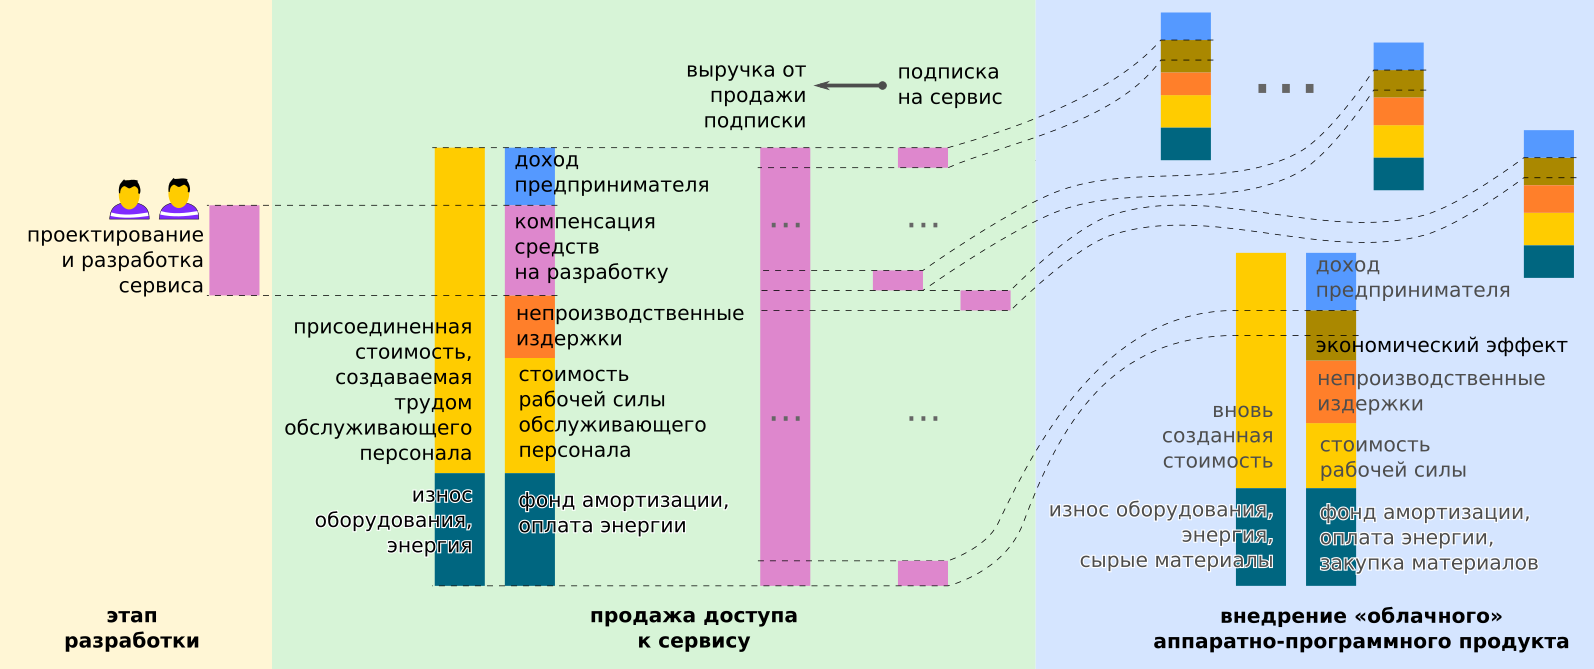
\includegraphics[width=0.95\textwidth]{model-eco-effect-saas}
    \caption{Компенсация расходов на разработку и функционирование аппаратно-программной платформы SaaS суммой долей экономических эффектов, реализованных внедрившими продукт потребителями}
    \label{fig:model_eco_effect_saas}
\end{figure}

С точки зрения потребителя услуги, если цена подписки окажется ниже экономического эффекта автоматизации, покупатель окажется в плюсе от подписки на сервис и внедрения его в свой производственный процесс, это будет являться для него объективным экономическим стимулом совершить покупку. Если для большинства потенциальных покупателей выгода от подписки окажется меньше её цены, запущенный сервис рискует остаться без потребителей.

Стоимость разработки ПО для облачного сервиса будет постепенно компенсирована из прибыли от продажи аппаратного обеспечения сервиса. Стоимость первоначального развертывания ПО на аппаратной платформе присоединяется к первоначальной стоимости аппаратного обеспечения и включается в продажную цену сервиса. Аппаратная инфраструктура не обязательно принадлежит непосредственно провайдеру сервиса, она может быть арендована им у третей стороны\footnote{«After making the decision to roll its own infrastructure and reduce its dependence on Amazon Web Services, Dropbox reduced its operating costs by \$74.6 million over the next two years» \cite{dropboxBuildsOwnInfra}}, дополнена необходимым программным обеспечением и в таком виде перепродана конечному потребителю.

Затратна предварительная разработка ПО. Для аппаратно"=программной платформы значительную часть кодовой базы можно взять из проектов с открытым исходным кодом или лицензировать у сторонних разработчиков. Некоторые проекты представляют открытые реализации программного обеспечения, готовые для развертывания и запуска сервиса целиком (например: WordPress, NextCloud, OnlyOffice), однако многие крупные игроки на рынке SaaS предпочитают использовать собственные закрытые разработки, работающие исключительно на их сервисах (например: DropBox, Яндекс Диск, MS Office 365), чтобы сохранять монопольное положение на рынке. Необходимость обслуживать большое количество клиентов в режиме 24/7 накладывает высокие требования к доступности и надежности сервиса. Ликвидация проблем и оптимизации могут требовать регулярных правок во внутреннюю кодовую базу на протяжении всего жизненного цикла проекта, их могут вносить сотрудники, совмещающие роль системных администратров и инженеров"=разработчиков\footnote{«Many important services in Google, e.g., Search, Ads, and Gmail, have dedicated teams of Site Reliability Engineers (SREs) responsible for the performance and reliability of these services. <...> The SRE teams are quite different from purely operational teams in that they place heavy emphasis on the use of engineering to approach problems.» \cite{googleSRE}}.

\section*{\raggedright{Продажа поддержки программного обеспечения}}

Эксплуатация программного обеспечения на собственной аппаратно"=программной инфраструктуре требует вовлечения труда технических специалистов — системных администраторов. Для потребителя ПО это выливается в известное количество эксплуатационных издержек, которые он несет на регулярной основе. В ряде ситуаций при решении этих задач может быть целесообразно заручиться помощью внешних специалистов: если настройка и эксплуатация программного продукта требует специальных знаний и навыков, не распространенных среди доступных на рынке труда специалистов и которыми не обладает имеющийся в штате специалист, если диагностика возможных проблем с программным пакетом требует развертывания специальной инфраструктуры разработки или доступ к закрытой кодовой базе и т.~п.

Производители программного обеспечения для автоматизации бизнеса кроме, собственно, программного пакета, могут предлагать клиентам дополнительные услуги с оплатой по подписке. Такая подписка обычно включает доступ к закрытым обновлениям ПО (критические обновления безопасности при этом могут публиковаться бесплатно), а также к службе поддержки\footnote{«Access to support engineers 24x7 for high-severity issues» \cite{redhatSubscriptionModel}}. Платные обновления — это форма коммерческого распространения программного обеспечения, по существу аналогичная модели продажи лицензий. Поддержка представляет собой возможность получать консультации специалистов компании-разработчика программного продукта.

Программный продукт может продаваться под отдельной коммерческой лицензией или распространяться бесплатно вместе с исходным кодом под свободной лицензией (хотя двоичные сборки свободного программного продукта могут быть формально не бесплатны, наличие исходного кода в открытом доступе позволяет получить из него исполняемый двоичный файл, идентичный коммерческой версии\footnote{«However, Ellison said that Oracle’s version would be identical with that of Red Hat.» \cite{oracleMovesToRedhat}}). Программное обеспечение в таком случае — разовая покупка или «бесплатное приложение» к труду людей, оплачиваемому на регулярной основе, повод купить повременной труд технических специалистов. Как и в случае с SaaS, успешная реализация модели приводит к сокращению необходимых издержек на обслуживание ИТ-инфраструктуры. Однако, в отличие от модели SaaS, аппаратная инфраструктура и обслуживающий персонал остаются внутри компании, а экономия достигается за счет повышения производительности труда администраторов системы, которые тратят меньше времени на решение проблем и реализацию специфических задач, получая консультации внешних оплаченных по подписке специалистов\footnote{«Finally, Red Hat Services has certified consultants available to accelerate your work and reduce time to value. These services can only be used in the context of a paid subscription.» \cite{redhatSubscriptionGuide}}.

Модель продажи поддержки ПО является действующей успешной моделью монетизации среди коммерческих компаний, распространяющих программные продукты вместе с открытым исходным кодом под свободной лицензией. При этом компания может являться непосредственным разработчиком программного продукта, вносить больший или меньший вклад в его разработку наряду с другими игроками или не вносить вклад в разработку, но предоставлять услуги по его обслуживанию и эксплуатации. В том случае, если компания несет издержки по разработке программного продукта, она их компенсирует из дохода от продажи поддержки.

\section*{\raggedright{Так называемые «интернет-сервисы»: Гугл, Яндекс, Ютюб, Твиттер, Телеграм и т.~п.}}

Технически интернет"=порталы, нацеленные на массовую аудиторию частных пользователей, такие, как поисковые системы, социальные сети, мессенджеры, хостинги видео, хостинги изображений, сервисы бесплатной электронной почты и т.~п. представляют собой серверную (облачную) аппаратно"=программную инфраструктуру с доступом через канал интернет через веб"=интерфейс или специализированное приложение, т.~е. по внешним признакам и технологиям реализации очень похожи на модель SaaS.

Однако, в отличие от модели SaaS, возможности таких интернет"=порталов доступны для массового пользователя бесплатно, между пользователем и порталом не возникает отношения купли"=продажи. Пользовательское соглашение обычно включает обязательства пользователя соблюдать правила портала, уведомление о том, что владелец портала может ограничить доступ пользователя к сервису в любой момент без объяснения причин, но не обязательства портала перед пользователем. Таким образом, хотя частные пользователи интернет"=порталов используют их программное обеспечение, аппаратные ресурсы и прочую серверную инфраструктуру для своих целей, нельзя говорить о том, что интернет-портал оказывает пользователю услугу (предоставляет сервис) — по крайней мере, с позиции экономических отношений.

Основная выручка крупнейших массовых интернет-порталов приходит по каналам рекламы. К примеру, выручка компании Фейсбук (в настоящее время — Мета, запрещена в РФ) в 2019 году составила \$70.697 млрд, из них от рекламы — \$69.655 млрд, чистый доход — \$18.485 млрд. \cite{facebook10K2019}. Таким образом, экономические отношения у массовых интернет-порталов возникают с рекламодателями — организациями, предлагающими пользователям портала через рекламные механизмы площадки свой продукт. Аппаратная серверная инфраструктура, энергия, канал связи, обслуживающий персонал, прочие операционные издержки текущей деятельности, а также первоначальные издержки на разработку программного обеспечения интернет-портала оплачены и компенсированы из средств рекламодателей, они же и являются его клиентами, т.~е. получателями услуги. Таким образом, массовые интернет-порталы (т.~н. интернет-сервисы) — это агрегированные по обществу непроизводственные издержки на рекламу.

С точки зрения рекламодателя выгода от использования интернет"=портала для размещения рекламы — сокращение собственных необходимых издержек на рекламу. Если купить рекламу у интернет"=портала окажется дешевле, чем содержать, к примеру, собственный отдел продаж, а отдача от такой рекламы окажется такая же или выше\footnote{«[Brandon Bateman] spent millions of dollars in Google and Facebook ad spend for his real estate investor clients over 2021 to generate leads and land deals. <...> Brandon says his clients typically do 10\% to 40\% bigger deals through digital marketing than physical marketing.» \cite{roiSEOvsGooglevsFacebook}}, то это будет объективным экономическим стимулом совершить покупку рекламы. Если же расходы на рекламу на выбранном портале в пересчете на реализованный продукт окажутся выше, чем такой же показатель для другого механизма обеспечения сбыта, покупать рекламу на таком портале будет экономически нецелесообразно\footnote{«Advertisers will not continue to do business with us if their investment in advertising with us does not generate sales leads, and ultimately customers, or if we do not deliver their advertisements in an appropriate and effective manner.» \cite{google10K2009}}.

Определение универсальной формулы для расчета стоимости размещения одного рекламного блока представляется крайне сложной, если вообще разрешимой задачей, т.~к. формы и механизмы размещения рекламы меняются со временем и от портала к порталу, в некоторых случаях они будут не вполне тривиальны. Но общий принцип заключается в том, что суммарная стоимость размещения от всех рекламодателей в выбранный период должна покрыть работу интернет-сервиса как аппаратно-программного комплекса — амортизацию оборудования, энергию, канал связи, работу обслуживающего персонала, прочие операционные расходы, — за этот же период времени. Первоначальные издержки на разработку ПО портала и прочие инвестиции будут компенсированы со временем из прибыли от текущей деятельности.

Наличие активной аудитории интернет-портала — необходимое условие для того, чтобы он имел возможность продавать рекламу. Для того, чтобы отдача от рекламы на портале была приемлемого уровня при приемлемой цене размещения, аудитория интернет-портала должна быть достаточно широка. В современном мире — это масштаб крупного государства или доли мирового рынка. После того, как портал уже запущен, он должен набрать достаточное количество пользователей — пройти период роста. К этому времени основные первоначальные издержки на разработку базового ПО и закупку аппаратной платформы уже понесены. В течение этого периода портал функционирует в полноценном режиме — потребляет энергию, связь, труд обслуживающего персонала, увеличение нагрузки может потребовать закупки дополнительного аппаратного обеспечения и расширения штата сотрудников. Но до тех пор, пока масса пользователей не достигла некоторого критического уровня, канал компенсации текущих расходов через продажу рекламы не открыт. Это дополнительные издержки, которые несут инвесторы проекта до тех пор, пока не начнет функционировать бизнес-модель, до выхода на окупаемость проект функционирует на средства инвесторов. Кроме расходов на текущую и расширяющуюся деятельность, привлечение аудитории требует значительных расходов на рекламу (рекламу самого сервиса на сторонних площадках). Период роста может занимать продолжительное время: обычная практика — несколько лет. В течение этого времени более важными показателями для инвесторов могут быть динамика роста и вовлечённость аудитории, чем текущие финансовые показатели такие, как выручка или прибыль.

Интернет-мессенджер с элементами социальной сети Телеграм был запущен основателем Павлом Дуровым в 2013 году \cite{telegramStartup2013}. Спустя два года — в 2015 году, — было объявлено о внедрении первых механизмов монетизации\footnote{«В мессенджере Telegram появятся платные сервисы от сторонних разработчиков. <...> Прибыль от платных приложений будет делиться между разработчиком и Telegram.» \cite{telegramMonetizationApps2015}} при активной аудитории 62 млн. человек \cite{telegramMonetizationApps2015}. Официальная платформа для рекламы в мессенджере была представлена в 2021 году\footnote{«вначале получаемые за рекламу деньги будет получать только сам мессенджер. Эти средства направят на обслуживание работы Telegram — покрытие затрат на оборудование и дата-центры.» \cite{telegramMonetizationAdvert2021}} — спустя 8 лет после запуска при количестве пользователей 500 млн.\footnote{«Сейчас у Telegram около 500 млн пользователей, а поддержка проектов такого масштаба, в том числе оплата расходов на серверы и трафик, обходится в “сотни миллионов долларов в год”, эти расходы уже невозможно оплачивать из личных сбережений» \cite{telegramAnnounceAdvert2020}} При том, что представленные механизмы (в т.~ч. появившиеся в 2022 премиальные аккаунты \cite{telegramPremium2022}) приносят значительный доход, по состоянию на март 2024 проект всё еще не вышел на полную самоокупаемость\footnote{«Дуров предположил, что Telegram может стать прибыльным сервисом уже в этом [2024] году. По его словам, мощный толчок к самоокупаемости сервиса в 2023 году дал запуск платной подписки Telegram Premium.» \cite{telegramIpoPlans2024}}, значит по-прежнему существует отчасти на средства инвесторов. По словам Дурова и по оценкам экспертов в 2015 году расходы на содержание серверной инфраструктуры составляли \$1 млн. в месяц\footnote{«До сих пор Павел Дуров оплачивал все расходы на работу сервиса из собственных средств. В июле 2015 года он оценил расходы на оборудование, персонал и транспорт примерно в \$1 млн в месяц.» \cite{telegramMonetizationApps2015}} (\$12 млн. в год), в 2020 году — \$275 млн. в год\footnote{«пока Telegram остается дотационным проектом. Его операционные расходы в 2020 г. составляли \$0,57 на пользователя, <...> так что исходя из объявленного количества пользователей текущие операционные затраты мессенджера можно оценить в \$275 млн ежегодно.» \cite{telegramIpoPlans2021}}, в 2024 году — \$630 млн. в год\footnote{«аудитория Telegram на текущий момент [март 2024] равна примерно 900 млн ежемесячно активных пользователей. Обслуживание каждого пользователя компании обходится в \$0,7 в год. Таким образом, на поддержание инфраструктуры Telegram ежегодно тратит около \$630 млн.» \cite{telegramIpoPlans2024}}. Мессенджер представлен в множестве стран мира, по состоянию на 2024 год больше всего закачек приложения происходит в Индии, России, Индонезии, США, Бразилии, Египте, Вьетнаме, Мексике, Украине \cite{telegramWorldStats2024}.

Особенность порталов, дающих возможность пользователям создавать или загружать в публичный доступ контент, — необходимость модерировать контент, как минимум для того, чтобы он не нарушал действующее законодательство\footnote{«In a statement posted to LinkedIn, Jean-Michel Bernigaud, secretary of France’s police agency focused on preventing violence against minors, confirmed Durov’s arrest and said it was related to the lack of moderation and cooperation of Telegram in fighting child sex crimes.» \cite{forbesDurovArrestModeration2024}}\footnote{«Telegram gave no details of the arrest but said the Dubai-based company abided by European Union laws and its moderation was “within industry standards and constantly improving”.» \cite{reutersDurovArrestModeration20224}}. Поэтому кроме системных администраторов облачную инфраструктуру на постоянной основе обслуживает команда контент-модераторов\footnote{«Facebook has 4,500 “content moderators” – and recently announced plans to hire another 3,000. <...> They [documents] show the breadth of the issues being dealt with by Facebook – from graphic violence to terrorism and cannibalism.» \cite{facebookModerators}}, стоимость рабочей силы которых присоединяется к стоимости издержек на содержание сервиса.

\section*{\raggedright{Смешанные модели: реклама vs SaaS}}

Многие массовые публичные интернет-сервисы, к примеру, Ютюб, Телеграм или Живой Журнал, получающие доход преимущественно за счет продажи рекламы, предоставляют своим пользователям возможность покупки платного (премиального) аккаунта. Некоторые сервисы, работающие по модели SaaS, получающие доход преимущественно за счет продажи аппаратных ресурсов, предоставляют своим пользователям возможность бессрочно работать с бесплатных аккаунтов, которые, однако, подразумевают показы рекламы (например: Gmail, Яндекс Диск). В рамках одного и того же сервиса часть пользователей, заплатившая за премиальные аккаунты, таким образом напрямую оплачивает потребляемые аппаратные ресурсы и прочую инфраструктуру. Стоимость оставшейся доли аппаратных ресурсов, потребляемой пользователями бесплатных аккаунтов, компенсируется рекламодателями по модели продажи рекламы. Обычная опция премиальных аккаунтов — отключение рекламы в платном режиме\footnote{«С подпиской YouTube Premium вам не придется прерываться на рекламу: мы не будем показывать вам объявления в начале и середине видео, а также оверлеи, сторонние баннеры и поисковые объявления.» \cite{youtubePremium}}\footnote{«Подписка стоит 499 руб. в месяц, пользователи могут загружать файлы до 4 ГБ и отключать рекламу. Дуров, анонсируя нововведение, говорил, что мессенджер “должен финансироваться в первую очередь пользователями”, а не рекламодателями» \cite{telegramPremium2022}}.

\section*{\raggedright{Портал Госуслуги}}

Портал Государственные услуги, как и прочие порталы взаимодействия граждан и специальных государственных учреждений и министерств (ФНС, ГИБДД), сайты муниципалитетов и т.~п., технически представляет собой аппаратно"=программную серверную инфраструктуру, аналогичную продуктам SaaS и порталам «бесплатных» массовых интернет"=сервисов. В отличие от модели SaaS, сам потребитель прямо не оплачивает доступ к порталу Госуслуг. В отличие от модели массовых интернет"=сервисов, портал Госуслуги не использует модель продажи рекламы для оплаты стоимости серверной инфраструктуры.

Функционирующий портал Госуслуг экономит время граждан\footnote{«Это позволит не только сэкономить деньги на “бумажном обороте”, но и время граждан, их транспортные расходы, отпадет необходимость брать отгулы за свой счет.» \cite{gosuslugiLaunch2009}}, а также повышает производительность труда государственных чиновников, это экономит государственный бюджет\footnote{АЦ при Правительстве РФ: «Подсчитано, что только сокращение издержек на содержание офисов для приема граждан и сокращение численности сотрудников, участвующих в оказании госуслуг при очном обращении, даст многомиллиардный эффект» \cite{gosuslugiCutExpenses2021}}, в этом заключается его прямой экономический эффект. Средства на его разработку и содержание выделяет общество в целом — через государственный бюджет, они составляют непроизводственные издержки в масштабах общества. Государственный бюджет покрывает как изначальные издержки на разработку ПО, так и текущие расходы на закупку, развертывание и содержание аппаратно-программной платформы и всей сопутствующей инфраструктуры портала с обслуживающим персоналом.

Запуск портала Госуслуги в России состоялся в 2009 году, на разработку его первой версии было потрачено 100 млн. рублей\footnote{«На создание портала понадобилось 100 миллионов рублей, из которых основные затраты ушли на создание центра обработки и хранения информации 20 тысяч территориальных органов.» \cite{gosuslugiLaunch2009}}. По информации, собранной фирмой «Победа права», затраты на разработку портала с 2013 по апрель 2023 года составили 16.9 млрд. рублей \cite{gosuslugiDevCostEstimate2023}. В 2019 году в России насчитывалось около 1.25 миллиона государственных и муниципальных чиновников\footnote{«По данным на 1 июля [2019], в стране порядка 855 тысяч государственных гражданских служащих. Из них 603 тысячи человек – федеральные гражданские служащие, 252 тысячи – гражданские служащие регионов. В органах местного самоуправления работают еще 395 тысяч муниципальных служащих.» \cite{minfinNumberOfOfficials2019}}, это составляет верхнюю границу потенциала экономии на рабочей силе в этом сегменте. Следует отметить, что интерфейс портала сам по себе сокращает время на подачу заявления и получения результата заявителем, но не на непосредственную обработку заявления по существу. Если в ведомстве, оказывающем услугу, не внедрен электронный документооборот, работа над поданными заявлениями подразумевает большой объем ручного труда, процедура оказания услуги останется неэффективной. Преждевременное сокращение штата исполнителей вместе с увеличившимся потоком заявлений в таком случае приведет к увеличению нагрузки на имеющийся персонал, качество оказания услуг при этом понизится. Для действительного повышения производительности добавление новых услуг на портал следует сопровождать внедрением внутренних средств автоматизации, облегчающих труд чиновников на местах. Инструменты такого рода также следует интегрировать с программными интерфейсами портала Госуслуги.

\section*{\raggedright{Частное потребление (b2c): игры}}

В настоящее время игровые программные продукты представлены на основных платформах: ПК, консоли, мобильные гаджеты, веб, аппаратно-программные платформы (игровые автоматы); и могут работать в рамках основных моделей: оффлайн-лицензия, оффлайн-подписка, SaaS, реклама, амортизация специализированного устройства (коллективное потребление игрового автомата).

Традиционная платформа для оффлайн-лицензий — ПК и консоли, с развитием рынка смартфонов и планшетов — мобильные гаджеты. Распространение специализированных магазинов приложений (маркетплейсов) на этих платформах облегчило процедуру покупки и доставки приложения на устройство пользователя, а также контроль за использованием лицензии для оффлайн-лицензии и оффлайн-подписки. По модели SaaS работают массовые многопользовательские онлайн игры, оплата серверной инфраструктуры может осуществляться как напрямую через платные аккаунты, так и косвенно — через «покупку» внутриигровых предметов\footnote{«Grand Theft Auto V's multiplayer mode GTA Online is free, but Rockstar offers optional microtransactions for players who want to speed up their progress. <...> As part of former Rockstar North president Leslie Benzies' \$150 million lawsuit against Take-Two, it's been revealed that GTA Online has generated “at least” \$500 million in revenue from microtransactions.» \cite{gtaOnlineHalfBillionMicrotrasacts}}. На мобильных гаджетах и веб-платформах для игр распространена смешанная модель: для «бесплатных» установок — реклама, альтернатива — покупка бессрочной или срочной лицензии, которая скрывает рекламу. Неделимой аппаратно-программной платформой, потребляемой коллективно, но в режиме оффлайн, являются игровые автоматы.

Особенность игрового сегмента заключается в том, что он нацелен в первую очередь на частное потребление, а не на бизнес. Игры не повышают производительность труда на производстве, не сокращают непроизводственные издержки, поэтому речи об экономических эффектах автоматизации здесь не идет. Источник ресурсов — кошелек частного потребителя. Стимул для покупки — субъективный пользовательский опыт, включающий впечатления от визуальной составляющей, игрового процесса, сюжета и т.~п. Важную роль играет мнение других игроков, масштаб и качество рекламной кампании.

Значительная часть предварительных издержек, кроме непосредственно разработки игры, — реклама перед запуском. Стоимость разработки дополнения «Phantom Liberty» к игре Cyberpunk 2077 составила \$62.8 миллионов при рекламном бюджете \$21.7 миллионов\footnote{«In total, over 3,600 people were involved in the game’s production in different capacities, out of which about 360 were core development staff.» \cite{cyberpunkMarketingBudget}}. Общий бюджет базовой версии игры Cyberpunk 2077 составил примерно \$316 миллионов\footnote{«While 530 developers from CD Projekt RED worked on the title, the total number of people “engaged” with the project was more than 5200. <...> This makes it one of the most expensive video games developed» \cite{cyberpunkTotalBudget}}, включая расходы на разработку и на рекламу. Хотя компания-разработчик CD Projekt не раскрыла соотношение расходов на разработку и рекламу для базовой версии игры, с учетом того, что рекламная кампания перед первоначальным запуском проходила в более интенсивном режиме, можно предположить, что в этом случае перевес был в большей степени в сторону рекламы (по одной из грубых оценок стоимость разработки могла составить от \$75 до \$120 миллионов \cite{cyberpunkDevBudgetEstimate}).

Конкуренты — другие игры (в аналогичном жанре или любом другом жанре, т.~к. вкусовые предпочтения одного потребителя могут варьироваться), любые другие продукты потребления и способы провождения свободного времени (выбор: «поиграть», «посмотреть фильм», «почитать книгу», «сходить в спортивный зал», «погулять», «просто отдохнуть»), инфляция, проценты по кредиту, стоимость услуг ЖКХ и т.~п.

Процесс разработки игры, кроме работы над программной составляющей, обычно включает необходимость создания игровых ресурсов — моделей, текстур, дизайна и наполнения уровней, музыки, звуковых эффектов, озвучки персонажей, прочего мультимедийного контента. Для больших проектов эта часть разработки может оказаться наиболее существенной по затратам. В части программной составляющей многие проекты используют готовые специализированные программные модули, фреймворки или платформы — т.~н. игровые «движки». Разработчики игровых движков могут распространять продукт среди разработчиков игр по разным моделям: например, для малых некоммерческих или учебных проектов предоставлять движок бесплатно, для коммерческих продуктов на стадии эксплуатации и продаж — продавать лицензию фиксированной стоимости или на условиях получения процента от продаж, а также дополнительно продавать к нему поддержку или включать её в цену лицензии.

Хотя финальная цена единичной копии игрового программного продукта не ограничена экономическим эффектом автоматизации, у частных потребителей могут сложиться определенные ценовые ожидания от продуктов разного уровня качества, попадающих в разные ценовые диапазоны (проекты уровня ААА — топовая графика, максимальное использование возможностей современного «железа»; средний ценовой диапазон, «независимые» «инди»-проекты, казуальные игры и т.~п.). Размер потенциальной аудитории можно оценить по данным о количестве пользователей целевых программных и аппаратно-программных платформ — десктоп, игровые приставки, мобильные устройства. Чем дороже разработка проекта, тем большую аудиторию потребуется привлечь, чтобы попасть в целевой ценовой диапазон и окупить издержки на разработку проекта и рекламу\footnote{«After eight years of development, Cyberpunk 2077 finally went out the door <...> CD Projekt said today that preorders alone were enough to earn back its development and marketing costs.» \cite{cyberpunkProfit}}, тем больше ресурсов необходимо вложить в первоначальную рекламную кампанию.

Потребитель может захотеть приобрести технологический продукт — программный пакет или аппаратно-программное устройство, — не только для получения субъективного опыта, но и с целью экономии собственного времени при выполнении повседневных личных или семейных дел: быт, общение, перемещение по городу. Повышение производительности такого рода будет являться объективным стимулом совершить покупку, хотя сэкономленное время при этом, однако, не получит прямого выражения в деньгах.

\section*{\raggedright{Прямое перераспределение стоимости с ИТ}}

Камеры дорожного наблюдения, прочие автоматические штрафы. Система камер дорожного наблюдения будет включать основные модули: распознавание объектов на дороге, дорожных ситуаций, номера авто (ИИ — специализированный программный алгоритм), система автоматического выписывания штрафов (интернет, ИТ-инфраструктура — база данных, программная логика приложения), аппаратная платформа (облачная инфраструктура, сеть уличных камер и т.~п.), обслуживающий персонал — операторы системы, системные администраторы и прочие.

Так же, как в случае с частным потреблением цифровых продуктов, источник ресурсов для компенсации исходных издержек на разработку и развертывание аппаратно-программной платформы и текущих операционных расходов — средства частных лиц\footnote{«В некоторых регионах, где система фиксации штрафов отдана частным компаниям, солидный процент остается у этих фирм, следящих за сохранностью оборудования и эксплуатирующих его. В одних регионах эти компании получают фиксированную сумму, другие - долю с каждого штрафа.» \cite{autoFineRF}}. Но, в отличие от игр и прочих программных продуктов, предназначенных для частного потребления, в рамках этой модели не требуется нести издержки на рекламу.

\section*{\raggedright{Добровольные пожертвования}}

В том случае, если разработчик программного продукта распространяет его бесплатно, в том числе с исходным кодом под свободной лицензией, при этом не применяет к нему рассмотренные или иные схемы коммерциализации, он все еще может полностью или частично компенсировать собственные издержки на разработку, принимая добровольные безвозмездные пожертвования без возникновения прямых обязательств перед отправляющей пожертвование стороной. Принимающая пожертвование сторона обычно — некоммерческие фонды, ассоциированные с проектами разработки свободного программного обеспечения (например, GNU FSF, Linux Foundation, Apache Software Foundation), или индивидуальные разработчики, получающие денежные переводы напрямую или через специализированную платформу (например, Patreon). Источник средств — частные лица («донаты») или корпоративные спонсоры. Пожертвования могут полностью или частично компенсировать издержки на разработку программного продукта или компенсировать сопутствующие расходы на инфраструктуру или деятельность, связанные с проектом, — оплата хостинга, проведение конференций, управление интеллектуальной собственностью, торговыми марками и т.~п.

Фонд Apache Software Foundation направляет собранные средства на оплату инфраструктуры, проведение мероприятий, управление интеллектуальной собственностью, но не на оплату труда разработчиков программного обеспечения\footnote{«All participants in ASF projects are volunteers and nobody (not even members or officers) is paid directly by the foundation to do their job. There are many examples of committers who are paid to work on projects, but never by the foundation itself.» \cite{apacheFunding}}. В 2023 году фондом было собрано \$2.294 млн., из них на поддержание инфраструктуры потрачено \$1.395 млн. \cite{apacheReport2023}. Фонд KDE e.V. оплачивает инфраструктуру, проводит для участников проекта конференции, хакатоны, кодспринты, которые позволяют вовлечь добровольцев в процесс разработки и обеспечить развитие кодовой базы на более-менее регулярной основе\footnote{«The goal of these sprints is to use face-to-face time to get work done in the most efficient way, and catalyze longer-term development efforts. <...> To support introduction and integration of new contributors into the community sprints are required to include new contributors.» \cite{kdeSprints}}. В 2022 году фонд израсходовал €384 тыс. на текущую деятельность, из них €68 тыс. на ежегодную конференцию Akademy, €14 тыс. на проведение спринтов, €12 тыс. на инфраструктуру, €209 тыс. на зарплату персоналу (10 человек), в этом же году фонд впервые открыл вакансии на инженерные позиции и нанял на них двух человек \cite{kdeeVReport2022}. Фонд FreeBSD Foundation кроме инфраструктуры и публичных мероприятий направляет часть собранных средств на непосредственную разработку проекта\footnote{«The FreeBSD Foundation supports both the development and popularization of FreeBSD» \cite{freeBsdAbout}}. В отчётах о проделанной работе среди спонсоров решений текущих задач указаны сам фонд, корпоративные спонсоры, также один из разработчиков получает персональное финансирование от частных лиц через платформу Patreon \cite{freeBsdStatus2023}. Некоммерческие фонды такого рода обычно позволяют корпоративным и частным спонсорам получать налоговые вычеты в государстве регистрации фонда\footnote{«As a charitable organization, the ASF is funded through tax-deductible contributions from corporations, foundations, and private individuals.» \cite{apacheHistory}}\footnote{«The KDE e.V. is accepted as a tax-exempt non-profit organization by the German financial authorities. That means that supporting membership fees are tax deductible for individuals and organizations residing in Germany.» \cite{kdeeVSupporting}}, таким образом фактически деятельность фондов частично спонсирует государство опосредованно через доноров, получающих вычеты.

Если оставить мотивы, не связанные напрямую с рассматриваемым программным продуктом, такие как альтруизм (со стороны частных лиц), получение налоговых вычетов или вложения в репутацию, т.~е. проведение пожертвования по линии рекламного бюджета, (со стороны корпоративных спонсоров) в стороне, объективным мотивом для пожертвования может быть желание получить новую улучшенную версию программного продукта\footnote{«Rather, companies or institutions that use the software and want to enhance it or maintain it provide the salary.» \cite{apacheFunding}}. Пожертвование может быть направлено на развитие проекта «в целом», или же целевым образом направлено на решение конкретной проблемы — исправление специфической ошибки или добавление определенной новой функции. В том случае, если необходимые новшества будут реализованы разработчиком проекта и войдут в очередной релиз программного продукта, спонсор проекта может частично или полностью окупить направленные им средства через реализацию экономического эффекта от внедрения в собственный производственный процесс улучшенной версии программного пакета. Т.~к. улучшенная версия продукта выпускается свободно в открытый доступ, экономический эффект в масштабах общества будет шире, чем частная выгода отправивших пожертвования спонсоров, — его смогут реализовать любые игроки, использующие программный продукт, в том числе те, кто не отправлял в проект пожертвования.

\section*{\raggedright{Смешанные модели: ОС Google Android}}

Программная часть для аппаратно-программной платформы — мобильных устройств — смартфонов и планшетов. Распространяется как свободное программное обеспечение. Значительная часть кодовой базы берется из общедоступного «фонда» свободного программного обеспечения (ядро Linux, программные библиотеки и т.~п.). Другая значительная часть — разработка корпорации Google, также публикуемая как свободное программное обеспечение. Производители устройств или типовых материнских плат берут базовую программную часть платформы как есть или вносят дополнительные доработки (добавляют закрытые драйверы устройств, брендируют под себя интерфейс)\footnote{«One part of the appeal is that, unlike other operating systems, Android is open source software, so anyone can use or change it. “We have access to the source code,” said Sanjay Jha, the co-chief executive of Motorola. “To do that on any other platform would be very difficult.”» \cite{windowsMobileVsAndroid2009}}\footnote{«Being a complete open source program, it also gave access to the device driver level code to the developers. That opened up some opportunity for the Device driver engineers if an OEM was looking to add/modify a default device driver of Android. <...> Most of the OEMs preferred to modify the vanilla Android and give some changed look and feel, which required re-skilling the developers in Android UI development.» \cite{androidChangedDeviceEngeneering2014}}, используют её в качестве базовой операционной системы собственных продуктов. Таким образом понижается потолок выхода на рынок нового устройства, по крайней мере, на него в меньшей степени оказывает влияние фактор необходимых издержек на разработку или лицензирование базовой программной прошивки\footnote{«It still costs a great deal of time and effort to build a great smartphone, but making a decent one is now easy. Android, even without any retouching or enhancements, is a first-class mobile OS, so all a manufacturer needs to do is figure out how to produce and sell the most attractive possible device at the cheapest possible price.» \cite{androidOemProfit2016}}.

Многие производители устройств вместе с операционной системой ставят на устройства пакет программ — сервисы Google. Google получает новых пользователей — покупателей смартфонов, привязанных к её бесплатным «сервисам» (поиск, почта, карты, Ютюб и т.~п.), замыкая на себя значительную долю мирового мобильного интернет-трафика\footnote{2024: «Over 60\% of website traffic comes from mobile devices.» \cite{mobileInternetTraffic2024}}. Основной источник дохода компании — реклама\footnote{Aplphabet (Google): «We generate a significant portion of our revenues from advertising. <...> We generated more than 75\% of total revenues from online advertising in 2023.» \cite{google10K2023}}\footnote{«Google Services generated revenue of \$253.53 billion for the 2022 fiscal year. That's about 90\% of its total revenue. <...> Google Services is thus the only segment that currently makes positive contributions to Alphabet's overall operating income.» \cite{investopediaGoogleBusiness}}. Таким образом, издержки на разработку бесплатной открытой операционной системы Google компенсирует из дохода от рекламы, который, в свою очередь, сохраняется и увеличивается благодаря тому, что мобильная операционная система, разрабатываемая компанией Google, доминирует на мобильном рынке. Доминирование, в свою очередь, в значительной степени обеспечено тем, что значительная доля необходимого программного обеспечения доступна производителям устройств бесплатно.

Хотя приложения — сервисы Google, — являются источником прибыли для компании Гугл, а значит сама компания заинтересована в том, чтобы они были установлены на максимальном количестве устройств, их наличие на устройстве, вместе с тем, является конкуретным преимуществом с точки зрения пользователя, оценивающего перед покупкой мобильное устройство\footnote{«Most internet use is now mobile, and YouTube occupies a huge chunk of our time while we’re on our phones, so any platform that’s missing a proper YouTube app is at a massive disadvantage.» \cite{windowsPhoneFailure2017}}\footnote{«This gives Huawei phones a very different, and less palatable, outlook.» \cite{androidHuaweiBan2019}}. Google может брать плату с производителей устройств в том числе за право предустановки своих сервисов. Информация о сделках такого рода обычно не публикуется, известные примеры в 2014 году — получение отчисления \$40 тыс. за партию 30 тыс. устройств, что составляло \$1.3 на устройство, отчисление \$75 тыс. за партию \$100 тыс. устройств, что составляло \$0.75 (75 центов) на устройство\footnote{«One source told the Guardian that the fee varies and is negotiated on a case-by-case basis, with one example costing \$40,000 for a batch of at least 30,000 devices. A separate source said that in another deal, a testing facility quoted \$75,000 to test 100,000 devices.» \cite{androidCosts2014}}.

По имеющимся данным, компания Майкрософт могла брать с производителей \$15 - \$25 за устройство за использование лицензии на ОС Windows Mobile\footnote{«Nevertheless, Android is free, while Windows Mobile costs manufacturers \$15 to \$25 a phone.» \cite{windowsMobileVsAndroid2009}}. В 2012 году представитель производителя ZTE сообщил, что они платят компании Майкрософт от £15 до £20 (от \$23 до \$31) за каждое устройство за использование ОС Windows Phone\footnote{«A ZTE executive has revealed to TrustedReviews that it costs between £15 and £20 for the company to license Windows Phone 7 from Microsoft.» \cite{zteWindowsPhoneOSCost2012}}. Линейка устройств с Windows Phone, производимых ZTE, на тот момент была представлена двумя смартфонами — Orbit (бюджетный вариант) и Tania (средняя ценовая категория) \cite{zteOrbitAndTania2012}. Розничную цену ZTE Orbit без дополнительных контрактов оператора, если они вообще были в свободной продаже, в настоящий момент в открытых источниках найти затруднительно. Розничная цена ZTE Tania в Великобритании составляла £250 (около \$357) \cite{zteTaniaPrice2012}. Если предположить, что £15 — это цена лицензии на ОС Windows Phone для устройств ZTE Orbit, а £20 — цена лицензии для устройств ZTE Tania, для смартфонов ZTE Tania цена лицензии на операционную систему составляла 8.7\% от его «базовой» (розничная цена за вычетом цены лицензии) цены\footnote{£20 / (£250 - £20) × 100 = 8.7\%}. В том случае, если такое же соотношение цены лицензии на ОС и «базовой» цены устройства справедливо для смартфонов ZTE Orbit, их розничная цена составила бы £187 (около \$268) за устройство\footnote{£15 / 8.7 × 100 + £15 = £187}, что довольно близко к нижней на тот момент ценовой планке устройств с ОС Windows Phone, составлявшей \$249. В 2013 году производитель Nokia объявил о выпуске нового самого бюджетного смартфона с Windows Phone — модели Nokia Lumia 520 с розничной ценой \$180\footnote{«Nokia has just announced <...> the Lumia 520, which pushes the price of Nokia’s Window Phone 8 devices to a new low of €139 (\$180) before taxes, down from its previous low of \$249.» \cite{androidPhoneLumia5202013}}. В 2014 году управляющий директор производителя Infosonics сообщил, что Майкрософт понижает цены на лицензии для производителей устройств на 70\%\footnote{«“We're hearing Microsoft will drop the license fee quite a bit, as far as 70 percent, which will make their product more competitive in terms of price,” Infosonics CEO Joseph Ram told PCMag» \cite{windowsPhoneLicense70Drop2014}}, это сообщение было интерпретировано журналистами как предоставление более выгодных  условий для существующих производителей\footnote{«Licensing fees for Windows Phone were between \$20 and \$30 as of the last word from a hardware partner, so a 70 percent cut would put new fees at roughly between \$6 and \$10 per unit.» \cite{windowsPhoneDiscountsTechcrunch2014}}. Однако в 2015 году появилась информация о новом разрабатываемом смартфоне с ОС Window Phone, который должен был установить новую нижнюю ценовую планку при цене \$55\footnote{«According to importation logs on Zauba the handset’s cost price is only 3,489 INR (around \$55) which would make it a new low for Windows Phone.» \cite{windowsPhone55USD2015}} (о ранней стадии переговоров стало известно в 2014 году\footnote{«You'll soon start to see low-cost Windows Phones appearing on re-used Android hardware. <...> Along with that, Microsoft announced a huge array of new hardware partners, including LG, Lenovo, and ZTE, as well as a bunch of Chinese and Indian vendors that are largely unknown in the U.S. like Gionee, Longcheer, and Xolo.» \cite{windowsPhoneLowCost2014}}). \$55 составляет почти ровно 30\% от \$180, т.~е. новое необъявленное официально устройство должно было стать на 70\% дешевле предыдущей самой дешевой модели. Таким образом, есть основания предполагать, что информация о «скидке» в 70\% со стороны Майкрософт в действительности могла означать фактическое предложение отдельному производителю более низкой цены на лицензию, абсолютное значение которой сократилось пропорционально сокращению «базовой» цены находящейся в разработке новой дешевой модели смартфона по сравнению с предыдущей самой дешевой моделью. При этом процентное отношение цены лицензии на ОС к «базовой» цене устройства осталось прежним и, опираясь на информацию от ZTE, могло составлять во всех случаях немногим менее 10\%.

В 2014 году розничная цена наиболее бюджетных моделей с ОС Android составляла около \$130 \cite{androidBudgetSmarphones2014}. Если взять максимальную из известных на тот момент комиссий Google за установку приложений доступа к своим сервисам \$1.3 на устройство, она бы составила 1\% от рассчитанной по аналогичной схеме «базовой» цены такого смартфона\footnote{\$1.3 / (\$130 - \$1.3) × 100 = 1\%}.

По расчетам исследователей Массачусетского университета в Амхерсте, усредненная общемировая норма прибыли после 2010 года могла составлять от 11\% до 23\% в зависимости от методики подсчета и выбранного набора данных \cite{worldProfitRates}. Если предположить, что в условиях жесткой конкуренции розничная цена смартфонов в это время устанавливалась из расчета минимальной нормы прибыли в 11\% на стоимость издержек производства аппаратной части, доля цены лицензии на ОС Windows Phone для смартфона ZTE Tania составила бы 80.7\% от расчетной прибыли\footnote{£250 / 111 × 11 = £24.77 — прибыль по норме 11\%; £20 / £24.77 × 100 = 80.7\%}. В случае со смартфонами на ОС Android, комиссия Google за установку своих сервисов при расчете на имеющихся данных с указанными допущениями по верхней планке могла составлять не более 10.1\% от рассчитанной таким образом прибыли производителя\footnote{\$130 / 111 × 11 = \$12.88 — прибыль по норме 11\%; \$1.3 / \$12.88 × 100 = 10.1\%}. При норме прибыли 23\% доля цены лицензии на ОС Microsoft Windows Phone составила бы 42.78\%\footnote{£250 / 123 × 23 = £46.75 — прибыль по норме 23\%; £20 / £46.75 × 100 = 42.78\%}, доля отчислений в пользу Google составила бы 5.35\%\footnote{\$130 / 123 × 23 = \$24.31 — прибыль по норме 23\%; \$1.3 / \$24.31 × 100 = 5.35\%}. При этом к возможности использовать кодовую базу операционной системы Google Android эти платежи прямо не относятся, производители, предпочитающие не устанавливать по умолчанию сервисы Google, могут использовать открытую версию операционной системы без всяких отчислений\footnote{«Huawei will no longer have access to Android apart from AOSP, the Android Open Source Project. This doesn’t require a license. Huawei can simply use it.» \cite{androidHuaweiBan2019}}, т.~е. получать в своё распоряжение всю прибыль от продажи аппаратной составляющей устройства.

Первые версии устройств с операционной системой Google Android были выпущены на рынок в сентябре 2008\footnote{«In September 2008, the very first Android smartphone was announced: the T-Mobile G1, also known as the HTC Dream in other parts of the world.» \cite{androidVersionHistory2024}}. Google купила компанию Android Inc. с ранней версией операционной системы в стадии разработки в 2005 году за \$50 млн.\footnote{«How much did Google buy Android for? The official documents state it was a mere \$50 million. <...> The Android team officially moved to Google’s campus in Mountain View, California on July 11, 2005. That day is considered the official date for the acquisition of Android by Google.» \cite{androidAquiredByGoogleHistory2022}} Общие расходы по статье исследования и разработки компании Google с 2005 по 2008 год составили \$6.74 млрд.\footnote{Ежегодные отчеты Google по форме 10-K (в тыс.): \$599,510 (2005) + \$1,228,589 (2006) + \$2,119,985 (2007) + \$2,793,192 (2008) = \$6,741,276 тыс. (\$6.74 млрд.) \cite{google10K2009}}, часть этих средств была потрачена на разработку ОС Android. Таким образом, первоначальная покупка и последующая разработка операционной системы до момента выпуска первой версии обошлась компании Google не более, чем в \$6.74 млрд. плюс \$50 млн. (\$6.79 млрд.). C 2009 по 2015 были выпущены версии операционной системы с 1.5 по 6.0 \cite{androidVersionHistory2024}, расходы на исследования и разработки в этот период составили \$47.8 млрд.\footnote{Отчеты Google 10-K (в млн.): \$2,843 (2009) + \$3,762 (2010) + \$5,162 (2011) + \$6,793 (2012) + \$7,137 (2013) + \$9,832 (2014) + \$12,282 (2015) = \$47,811 (\$47.8 млрд.) \cite{google10K2009, google10K2012, google10K2015}} Выручка компании Google от рекламы только на мобильных устройствах после вычета партнерских комиссий в 2017 году могла составить около \$50 млрд. (67\% от чистой общей рекламной выручки), в 2016 — \$38 млрд.\footnote{«Nearly \$50 billion, or 67 percent of Google’s net digital ad revenue, will come from mobile in 2017, up from \$38 billion in 2016, according eMarketer.» \cite{googleRevenue2017}} (61\% от чистой общей рекламной выручки\footnote{Выручка Google от рекламы за вычетом партнерских комиссиий за покупку трафика в 2016: \$79,38 млрд. - \$16.79 млрд. = \$62.59 млрд. \cite{google10K2017}; доля мобильной выручки в чистой общей выручке за рекламу в 2016: \$38 млрд. / \$62.59 млрд. × 100 = 61\%}). Таким образом, выручка компании от мобильной рекламы за один 2017 год превысила издержки на разработку первой версии операционной системы до момента релиза и, скорее всего, издержки на разработку всех новых версий до 2016 года. Общая выручка от мобильной рекламы за 2016 и 2017 годы (\$88 млрд.\footnote{\$38 млрд. + \$50 млрд. = \$88 млрд.}) превысила все возможные издержки на разработку операционной системы до 2016 года при их максимальной оценке (\$54.59 млрд.\footnote{\$6.79 млрд. млрд. + \$47.8 млрд. = \$54.59 млрд.}) с заметным запасом.

Рост доли рынка в том числе за счет нового мобильного трафика увеличивает нагрузку на аппаратную инфраструктуру компании\footnote{«Other cost of revenues increased \$5,566 million from 2016 to 2017. The increase was due to various factors, including an increase in data center and other operations costs, which include depreciation, <...>, energy, bandwidth, and other equipment costs as a result of business growth» \cite{google10K2017}}. В отчетах компании Google расходы на датацентры прямо не детализируются, но среди прочих расходов входят в статью «прочие компоненты себестоимости выручки» («other cost of revenues»). Расходы по этой статье увеличились с \$2.67 млрд. в 2009 году\footnote{Прочие компоненты себестоимости выручки Google (себестоимость выручки за вычетом партнерских комиссий за покупку трафика) в 2009: \$8.84 млрд. - \$6.17 млрд. = \$2.67 млрд. \cite{google10K2009}} до \$18.35 млрд. в 2016 и \$23.91 млрд. в 2017 \cite{google10K2017}. Таким образом, выручка от одной мобильной рекламы только в 2016 и 2017 годах превысила расходы на содержание всей аппаратной инфраструктуры компании при их максимальной оценке за это же время. Если же взять долю оцененных таким образом издержек на содержание аппаратной инфраструктуры пропорциональную доле выручки от мобильной рекламы в общей выручке от всей рекламы (\$27 млрд.\footnote{\$18.35 / 100 × 61=\$11.19 млрд. (2016); \$23.91 / 100 × 67 = \$16.02 млрд. (2017); \$11.19 млрд. + \$16.02 млрд. = \$27.21 млрд}), то общая выручка от одной мобильной рекламы в 2016 и 2017 годы после вычета партнерских комиссий превысит расходы на содержание соответствующей доли аппаратной инфраструктуры компании за этот же период и весь бюджет исследований и разработок компании с 2005 по 2015 год, а, значит, и бюджет на разработку ОС Android, взятые вместе.

Таким образом, разработка и развитие ОС Google Android, как и значительная доля всех интеллектуальных разработок и аппаратной инфраструктуры компании Google, в конечном итоге в масштабах всей мировой экономики оплачены долей экономического эффекта сокращения необходимых непроизводственных издержек на организацию сбыта производимых мировой фабрикой продуктов, т.~е. мировых издержек на рекламу.

% чтобы ссылки в тексте имели правильные номера, генератор нужно запустить два раза
% нижние подчеркивания '_' в ссылках заменяем на '\_', иначе они воспринимаются как спец-символы
\begin{thebibliography}{2}
\bibitem{ecoEffects} Моисеев, А.~Е. Оценка эффективности цифровой трансформации секторов экономики / А.~Е.~Моисеев, Н.~А.~Мурашова // Инновации и инвестиции. – 2023. – № 7. – С. 388-391. – EDN IXZPSY.
\bibitem{driscollOpenLetter} Driscoll, Kevin. «Professional Work for Nothing: Software Commercialization and “An Open Letter to Hobbyists”.» Information \& Culture: A Journal of History, vol. 50 no. 2, 2015, p. 257-283. Project MUSE, \url{https://doi.org/10.1353/lac.2015.0005}
\bibitem{phoneUpdates} Here are the phone update policies from every major Android manufacturer / C.~Scott Brown // Android Authority, – 2023. [Электронный ресурс]. – URL: \url{https://www.androidauthority.com/phone-update-policies-1658633/}
\bibitem{microsoftPiracyReinvest} Q\&A: How Software Piracy Undermines Economic Recovery / Nancy Anderson // PressPass, – 2001. [Электронный ресурс]. – URL: \url{https://news.microsoft.com/2001/10/19/qa-how-software-piracy-undermines-economic-recovery/}
\bibitem{facebookCassandra} Out in the Open: The Abandoned Facebook Tech That Now Helps Power Apple / Klint Finley // Wired, – 2014. [Электронный ресурс]. – URL: \url{https://www.wired.com/2014/08/datastax/}
\bibitem{yandexYDB} Яндекс выложил в опенсорс YDB / Пресс-служба Яндекса // Яндекс, – 2022. [Электронный ресурс]. – URL: \url{https://yandex.ru/company/news/2022-04-19}
\bibitem{yandexClickHouse} «Яндекс» решил сделать свою открытую СУБД коммерческой, потратив на проект \$50 млн / Дарья Лебедева // CNews, – 2021. [Электронный ресурс]. – URL: \url{https://www.cnews.ru/news/top/2021-09-21\_yandeks\_szaregistriroval}
\bibitem{googleTensorFlow} Google Just Open Sourced TensorFlow, Its Artificial Intelligence Engine / Cade Metz // Wired, – 2015. [Электронный ресурс]. – URL: \url{https://www.wired.com/2015/11/google-open-sources-its-artificial-intelligence-engine/}
\bibitem{rosneftSoft} «Роснефть» презентовала нефтегазовым компаниям новое программное обеспечение // ComNews, – 2024. [Электронный ресурс]. – URL: \url{https://www.comnews.ru/content/232818/2024-04-22/2024-w17/1010/rosneft-prezentovala-neftegazovym-kompaniyam-novoe-programmnoe-obespechenie}
\bibitem{mintcifriForbidInhouseSoft} Минцифры хочет запретить госкомпаниям разработку дублирующего софта / Анна Устинова // Ведомости, – 2024. [Электронный ресурс]. – URL: \url{https://www.vedomosti.ru/technology/articles/2024/05/29/1040118-mintsifri-hochet-zapretit-goskompaniyam-razrabotku-dubliruyuschego-softa}
\bibitem{accountingIAS} Международный стандарт финансовой отчетности (IAS) 38 «Нематериальные активы» // Минфин России, – 2023. [Электронный ресурс]. – URL: \url{https://minfin.gov.ru/ru/document/?id\_4=15329}
\bibitem{accountingNKRF257} НК РФ Статья 257. Порядок определения стоимости амортизируемого имущества. П.3.: нематериальные активы. // Налоговый кодекс РФ, – 2023. [Электронный ресурс]. – URL: \url{https://www.consultant.ru/document/cons\_doc\_LAW\_28165/cf1a9426ba878faee9824672bca283c1420a2b1e/}
\bibitem{accountingNKRF264} НК РФ Статья 264. Прочие расходы, связанные с производством и (или) реализацией. П.26.: расходы, связанные с приобретением права на использование программ для ЭВМ и баз данных по договорам с правообладателем (по лицензионным и сублицензионным соглашениям) // Налоговый кодекс РФ, – 2023. [Электронный ресурс]. – URL: \url{https://www.consultant.ru/document/cons\_doc\_LAW\_28165/3fdee9a04c76f1af1e084502759523cd77da7d16/}
\bibitem{introToDigital} Introduction to Digital Economics: Foundations, Business Models and Case Studies / Harald Øverby, Jan Arild Audestad // Springer Cham. – 2021. – С. 78-80. – DOI 10.1007/978-3-030-78237-5. – eBook ISBN 978-3-030-78237-5.
\bibitem{windowsXPLegacy} Microsoft begs users to leave Windows XP – gives them until 2014 to do it / Jeffrey Van Camp // Digital Trends, – 2011. [Электронный ресурс]. – URL: \url{https://www.digitaltrends.com/computing/microsoft-begs-users-to-leave-windows-xp-gives-them-until-2014-to-do-it/}
\bibitem{autodeskSubscription} Using Autodesk subscription products without an internet connection // Autodesk, – 2023. [Электронный ресурс]. – URL: \url{https://www.autodesk.com/support/technical/article/caas/sfdcarticles/sfdcarticles/About-using-a-Autodesk-product-on-subscription-without-an-Internet-connection.html}
\bibitem{microsoftInvestsRF} За три года Microsoft инвестирует в Россию 10 млрд руб. / Татьяна Короткова // CNews, – 2009. [Электронный ресурс]. – URL: \url{https://www.cnews.ru/news/line/za\_tri\_goda\_microsoft\_investiruet\_v}
\bibitem{cloudIsAFancyName} Disrupting Nation State Hackers / Rob Joyce // USENIX Association, – 2016. [Электронный ресурс]. – URL: \url{https://www.usenix.org/conference/enigma2016/conference-program/presentation/joyce}
\bibitem{saasVsPerpetualLicense} Why is Cloud Licensing (SaaS) Replacing Perpetual Licenses? / Kumiko Saito // Kivuto, – 2022. [Электронный ресурс]. – URL: \url{https://kivuto.com/blog/why-is-cloud-licensing-saas-replacing-perpetual-licenses/}
\bibitem{subscriptionProspere} 5 Companies That Prospered With Subscriptions / Matthew Lekoutovich // eLabs, – 2022. [Электронный ресурс]. – URL: \url{http://web.archive.org/web/20221207025045/https://elabsinc.com/5-companies-that-thrived-with-subscriptions/}
\bibitem{microsoftMoveToSubscriptionAndSaas} Microsoft's move to Subscription and SaaS / David Foxen // ITAM Review, – 2015. [Электронный ресурс]. – URL: \url{https://itassetmanagement.net/2015/06/02/microsofts-move-subscription-saas/}
\bibitem{microsoftAzureAnnounce2008} Microsoft Unveils Windows Azure at Professional Developers Conference // Microsoft, – 2008. [Электронный ресурс]. – URL: \url{https://news.microsoft.com/2008/10/27/microsoft-unveils-windows-azure-at-professional-developers-conference/}
\bibitem{google10K2009} Google Inc., Form 10-K: Annual report for the fiscal year ended December 31, 2009 // U.S. Securities and Exchange Commission, – 2010. [Электронный ресурс]. – URL: \url{https://www.sec.gov/Archives/edgar/data/1288776/000119312510030774/d10k.htm}
\bibitem{dataCenters2021} Microsoft, Amazon, and Google operate half the world’s 600 hyperscale data centers / Dan Swinhoe // Data Centre Dynamics, – 2021. [Электронный ресурс]. – URL: \url{https://www.datacenterdynamics.com/en/news/microsoft-amazon-and-google-operate-half-the-worlds-600-hyperscale-data-centers/}
\bibitem{saasEnegry2021} Microsoft Teams Up With Accenture, Goldman on Greener Software / Dina Bass // Bloomberg, – 2021. [Электронный ресурс]. – URL: \url{https://www.bloomberg.com/news/articles/2021-05-25/microsoft-teams-up-with-accenture-goldman-on-greener-software}
\bibitem{googleDutchDataCenter2016} From day one, Dutch data center matched with 100\% locally-sourced renewable energy // Google, – 2016. [Электронный ресурс]. – URL: \url{https://blog.google/around-the-globe/google-europe/dutch-datacenter-google-100-renewable-energy/}
\bibitem{dataCentersNeedStaff2021} Data centers need to find 300,000 more staff by 2025 / Peter Judge // Data Centre Dynamics, – 2021. [Электронный ресурс]. – URL: \url{https://www.datacenterdynamics.com/en/news/data-centers-need-find-300000-more-staff-2025/}
\bibitem{erpSaas} The future of business ERP is SaaS. Reporting from Directions EMEA 2021 // LS Retail, – 2021. [Электронный ресурс]. – URL: \url{https://www.lsretail.com/resources/the-future-of-business-erp-is-saas-reporting-from-directions-emea-2021}
\bibitem{sellingServices} How to Shift from Selling Products to Selling Services / Doug J.~Chung // Harvard Business Review, – 2021. [Электронный ресурс]. – URL: \url{https://hbr.org/2021/03/how-to-shift-from-selling-products-to-selling-services}
\bibitem{dropboxBuildsOwnInfra} Dropbox saved almost \$75 million over two years by building its own tech infrastructure / Tom Krazit // GeekWire, – 2018. [Электронный ресурс]. – URL: \url{https://www.geekwire.com/2018/dropbox-saved-almost-75-million-two-years-building-tech-infrastructure/}
\bibitem{googleSRE} Being an On-Call Engineer: A Google SRE Perspective / Andrea Spadaccini, Kavita Guliani // ;login:, vol. 40 no. 5, p. 43-47., – 2015. [Электронный ресурс]. – URL: \url{https://www.usenix.org/publications/login/oct15/spadaccini}
\bibitem{redhatSubscriptionModel} Red Hat subscription model FAQ: What's included in a subscription? // Red Hat, – 2023. [Электронный ресурс]. – URL: \url{https://www.redhat.com/en/about/subscription-model-faq}
\bibitem{oracleMovesToRedhat} Oracle makes its move on Red Hat / ITP Staff // edge, – 2006. [Электронный ресурс]. – URL: \url{https://www.edgemiddleeast.com/news/488113-oracle-makes-its-move-on-red-hat}
\bibitem{redhatSubscriptionGuide} Red Hat Enterprise Linux subscription guide // Red Hat, – 2023. [Электронный ресурс]. – URL: \url{https://www.redhat.com/en/resources/red-hat-enterprise-linux-subscription-guide}
\bibitem{facebook10K2019} Facebook, Inc., Form 10-K: Annual report for the fiscal year ended December 31, 2019 // U.S. Securities and Exchange Commission, – 2020. [Электронный ресурс]. – URL: \url{https://www.sec.gov/ix?doc=/Archives/edgar/data/1326801/000132680120000013/fb-12312019x10k.htm}
\bibitem{roiSEOvsGooglevsFacebook} \$1.2 Million Spent on Ads | Comparing ROI SEO vs. Google Ads vs. Facebook Ads for Real Estate Investors / Mike Blankenship // carrot, – 2022. [Электронный ресурс]. – URL: \url{https://carrot.com/blog/facebook-ads-vs-google-ads-vs-seo-for-real-estate-investors/}
\bibitem{telegramStartup2013} Телеграмма от Дурова / Роман Дорохов // Ведомости, – 2013. [Электронный ресурс]. – URL: \url{https://www.vedomosti.ru/newspaper/articles/2013/08/15/telegramma-ot-durova}
\bibitem{telegramMonetizationApps2015} Как Павел Дуров заработает на бесплатном Telegram / Виталий Алексеев // Деловой Петербург, – 2015. [Электронный ресурс]. – URL: \url{https://www.dp.ru/a/2015/09/22/Pavel\_Durov\_monetiziruet}
\bibitem{telegramMonetizationAdvert2021} Telegram представил официальную платформу для рекламы в мессенджере / Георгий Тадтаев // РБК, – 2021. [Электронный ресурс]. – URL: \url{https://www.rbc.ru/technology\_and\_media/26/10/2021/617826fd9a79473a3ecf7b27}
\bibitem{telegramAnnounceAdvert2020} Дуров объявил о начале монетизации Telegram. Что важно знать / Евгений Калюков, Владислав Скобелев, Анастасия Скрынникова // РБК, – 2020. [Электронный ресурс]. – URL: \url{https://www.rbc.ru/technology\_and\_media/23/12/2020/5fe2f84b9a79475d08f5a503}
\bibitem{telegramPremium2022} Telegram запустил платную подписку Premium / Наталия Анисимова // РБК, – 2022. [Электронный ресурс]. – URL: \url{https://www.rbc.ru/technology\_and\_media/19/06/2022/62af7fd69a79477c87b3a8a4}
\bibitem{telegramIpoPlans2024} Павел Дуров рассказал, сколько стоит Telegram / Роман Кильдюшкин // газета.ru, – 2024. [Электронный ресурс]. – URL: \url{https://www.gazeta.ru/tech/news/2024/03/11/22524997.shtml}
\bibitem{telegramIpoPlans2021} Telegram планирует провести IPO в течение двух лет / Тимур Бордюг // Ведомости, – 2021. [Электронный ресурс]. – URL: \url{https://www.vedomosti.ru/media/articles/2021/04/11/865492-telegram-planiruet-provesti-ipo}
\bibitem{telegramWorldStats2024} Telegram Users by Country 2024 // World Population Review, – 2024. [Электронный ресурс]. – URL: \url{https://worldpopulationreview.com/country-rankings/telegram-users-by-country}
\bibitem{forbesDurovArrestModeration2024} Officials Confirm Arrest Of Billionaire Telegram CEO Pavel Durov In France: Here’s What We Know / Molly Bohannon // Forbes, – 2024. [Электронный ресурс]. – URL: \url{https://www.forbes.com/sites/mollybohannon/2024/08/26/officials-confirm-arrest-of-billionaire-telegram-ceo-pavel-durov-in-france-heres-what-we-know/}
\bibitem{reutersDurovArrestModeration20224} Telegram CEO arrested over probe into child porn, drug trafficking on app / Layli Foroudi, Tassilo Hummel // Reuters, – 2024. [Электронный ресурс]. – URL: \url{https://www.reuters.com/world/europe/pavel-durov-has-nothing-hide-telegram-says-arrested-founder-2024-08-26/}
\bibitem{facebookModerators} Facebook moderators: a quick guide to their job and its challenges / Nick Hopkins // The Guardian, – 2017. [Электронный ресурс]. – URL: \url{https://www.theguardian.com/news/2017/may/21/facebook-moderators-quick-guide-job-challenges}
\bibitem{youtubePremium} Какие возможности дает YouTube Premium // Google, – 2023. [Электронный ресурс]. – URL: \url{https://support.google.com/youtube/answer/6308116}
\bibitem{gosuslugiLaunch2009} Состоялся запуск интернет-портала госуслуг / Мария Жебит, Татьяна Шадрина // Российская газета, – 2009. [Электронный ресурс]. – URL: \url{https://rg.ru/2009/12/15/gosuslugi-portal-site.html}
\bibitem{gosuslugiCutExpenses2021} Чернышенко: услуги по оформлению справок и пособий будут оказываться к 2024 году онлайн // ТАСС, – 2021. [Электронный ресурс]. – URL: \url{https://tass.ru/ekonomika/12609239}
\bibitem{gosuslugiDevCostEstimate2023} Стоимость «Госуслуг»: сколько тратят на портал и его развитие // «Победа права», – 2023. [Электронный ресурс]. – URL: \url{https://dzen.ru/a/ZFEJbPapQCu8fKdH}
\bibitem{minfinNumberOfOfficials2019} В Минфине назвали число чиновников в России / Наталья Селиверстова // РИА Новости, – 2019. [Электронный ресурс]. – URL: \url{https://ria.ru/20190923/1558989134.html}
\bibitem{gtaOnlineHalfBillionMicrotrasacts} GTA 5's Online Mode Has Generated Half a Billion Dollars - Report / Eddie Makuch // GameSpot, – 2016. [Электронный ресурс]. – URL: \url{https://www.gamespot.com/articles/gta-5s-online-mode-has-generated-half-a-billion-do/1100-6438765/}
\bibitem{cyberpunkMarketingBudget} Cyberpunk 2077: Phantom Liberty Had a Development and Marketing Budget of Nearly \$85 Million / Shubhankar Parijat // GamingBolt, – 2023. [Электронный ресурс]. – URL: \url{https://gamingbolt.com/cyberpunk-2077-phantom-liberty-had-a-development-and-marketing-budget-of-nearly-85-million}
\bibitem{cyberpunkTotalBudget} Cyberpunk 2077’s Total Budget Was Roughly \$316 Million / Ravi Sinha // GamingBolt, – 2021. [Электронный ресурс]. – URL: \url{https://gamingbolt.com/cyberpunk-2077s-total-budget-was-roughly-316-million}
\bibitem{cyberpunkDevBudgetEstimate} Cyberpunk 2077 Budget: How much did it cost to make the game? / Hrithik Raj // Sportskeeda, – 2020. [Электронный ресурс]. – URL: \url{https://www.sportskeeda.com/esports/cyberpunk-2077-budget-how-much-cost-make-game}
\bibitem{cyberpunkProfit} After eight years of development, Cyberpunk 2077 made a profit in one day /Andy Chalk // PC Gamer, – 2020. [Электронный ресурс]. – URL: \url{https://www.pcgamer.com/after-eight-years-of-development-cyberpunk-2077-made-a-profit-in-one-day/}
\bibitem{autoFineRF} Куда и на что уходят автомобильные штрафы / Майя Бирюкова // Российская газета, – 2020. [Электронный ресурс]. – URL: \url{https://rg.ru/2020/09/03/kuda-i-na-chto-uhodiat-avtomobilnye-shtrafy.html}
\bibitem{apacheFunding} How the ASF works // Apache Software Foundation (ASF), – 2024. [Электронный ресурс]. – URL: \url{https://www.apache.org/foundation/how-it-works/}
\bibitem{apacheReport2023} The Apache Software Foundation - Annual Report - FY2023 // Apache Software Foundation (ASF), – 2023. [Электронный ресурс]. – URL: \url{https://apache.org/foundation/docs/FY2023AnnualReport.pdf}
\bibitem{kdeSprints} KDE Sprint Policy // KDE e.V., – 2024. [Электронный ресурс]. – URL: \url{https://ev.kde.org/rules/sprint\_policy/}
\bibitem{kdeeVReport2022} KDE e.V. COMMUNITY REPORT, 2022, Issue 39 // KDE e.V., – 2023. [Электронный ресурс]. – URL: \url{https://ev.kde.org/reports/ev-2022/}
\bibitem{freeBsdAbout} About the Foundation // FreeBSD Foundation, – 2023. [Электронный ресурс]. – URL: \url{https://freebsdfoundation.org/about-us/about-the-foundation/}
\bibitem{freeBsdStatus2023} FreeBSD Status Report Fourth Quarter 2023 // FreeBSD Foundation, – 2023. [Электронный ресурс]. – URL: \url{https://www.freebsd.org/status/report-2023-10-2023-12/}
\bibitem{apacheHistory} History of the Apache Software Foundation // Apache Software Foundation (ASF), – 2024. [Электронный ресурс]. – URL: \url{https://www.apache.org/history/}
\bibitem{kdeeVSupporting} Become a Supporting Member of the KDE e.V. // KDE e.V., – 2020. [Электронный ресурс]. – URL: \url{https://ev.kde.org/getinvolved/supporting-members/}
\bibitem{windowsMobileVsAndroid2009} Big Cellphone Makers Shifting to Android System / Saul Hansell // The New York Times, – 2009. [Электронный ресурс]. – URL: \url{https://www.nytimes.com/2009/10/26/technology/26android.html}
\bibitem{androidChangedDeviceEngeneering2014} How did Android Change the Mobile Device Engineering business? / Subhamoy C. // LinkedIn Pulse, – 2014. [Электронный ресурс]. – URL: \url{https://www.linkedin.com/pulse/20140705181714-5022498-how-did-android-change-the-mobile-device-engineering-business}
\bibitem{androidOemProfit2016} Why do profit-seeking companies keep making profitless Android phones? / Vlad Savov // The Verge, – 2016. [Электронный ресурс]. – URL: \url{https://www.theverge.com/2016/2/3/10894200/android-smartphone-oem-profit}
\bibitem{mobileInternetTraffic2024} Internet Traffic from Mobile Devices (Jun 2024) / Josh Howarth // Exploding Topics, – 2024. [Электронный ресурс]. – URL: \url{https://explodingtopics.com/blog/mobile-internet-traffic}
\bibitem{google10K2023} Alphabet Inc., Form 10-K: Annual report for the fiscal year ended December 31, 2023 // U.S. Securities and Exchange Commission, – 2024. [Электронный ресурс]. – URL: \url{https://www.sec.gov/ix?doc=/Archives/edgar/data/1652044/000165204424000022/goog-20231231.htm}
\bibitem{investopediaGoogleBusiness} How Google (Alphabet) Makes Money: Advertising and Cloud / Matthew Johnston // Investopedia, – 2023. [Электронный ресурс]. – URL: \url{https://www.investopedia.com/articles/investing/020515/business-google.asp}
\bibitem{windowsPhoneFailure2017} Windows Phone was a glorious failure / Vlad Savov // The Verge, – 2017. [Электронный ресурс]. – URL: \url{https://www.theverge.com/2017/10/10/16452162/windows-phone-history-glorious-failure}
\bibitem{androidHuaweiBan2019} What Google's Huawei ban means for millions of Android owners / Andrew Williams // Wired, – 2019. [Электронный ресурс]. – URL: \url{https://www.wired.com/story/huawei-google-ban-uk-android/}
\bibitem{androidCosts2014} The hidden costs of building an Android device / Charles Arthur, Samuel Gibbs // The Guardian, – 2014. [Электронный ресурс]. – URL: \url{https://www.theguardian.com/technology/2014/jan/23/how-google-controls-androids-open-source}
\bibitem{zteWindowsPhoneOSCost2012} ZTE Pays Microsoft £15-£20 Per Phone / David Gilbert // TrustedReviews, – 2012. [Электронный ресурс]. – URL: \url{http://web.archive.org/web/20120302135323/http://www.trustedreviews.com/news/zte-pays-microsoft-15-20-per-phone}
\bibitem{zteOrbitAndTania2012} Hands-on With ZTE’s Inexpensive Windows Phones / Ginny Mies // PCWorld, – 2012. [Электронный ресурс]. – URL: \url{https://www.pcworld.com/article/468640/zte\_goes\_for\_affordability\_with\_its\_windows\_phones\_we\_go\_for\_the\_hands\_on.html}
\bibitem{zteTaniaPrice2012} ZTE launches its first Windows phone / Charles McLellan // ZDNET, – 2012. [Электронный ресурс]. – URL: \url{https://www.zdnet.com/article/zte-launches-its-first-windows-phone/}
\bibitem{androidPhoneLumia5202013} Nokia Expands Its Windows Phones To More Price Points With \$180 Entry Level Lumia 520 And \$330 Mid-Range Lumia 720 / Natasha Lomas // TechCrunch, – 2013. [Электронный ресурс]. – URL: \url{https://techcrunch.com/2013/02/24/nokia-expands-its-windows-phones-to-more-price-points-with-180-entry-level-lumia-520-and-330-mid-range-lumia-720/}
\bibitem{windowsPhoneLicense70Drop2014} OEM: Windows Phone License Fee Plummeting / Sascha Segan // PCMag, – 2014. [Электронный ресурс]. – URL: \url{https://www.pcmag.com/news/oem-windows-phone-license-fee-plummeting}
\bibitem{windowsPhoneDiscountsTechcrunch2014} Microsoft Could Slash Windows Phone Licensing Fees By Up To 70\% To Take On Low-Cost Androids / Darrell Etherington // TechCrunch, – 2014. [Электронный ресурс]. – URL: \url{https://techcrunch.com/2014/02/26/microsoft-could-slash-windows-phone-licensing-fees-by-up-to-70-to-take-on-low-cost-androids/}
\bibitem{windowsPhone55USD2015} With \$55 Windows Phone Microsoft is getting ready to replace their feature phone business / Surur Davids // MSPowerUser, – 2015. [Электронный ресурс]. – URL: \url{https://mspoweruser.com/with-55-windows-phone-microsoft-is-getting-ready-to-replace-their-feature-phone-business/}
\bibitem{windowsPhoneLowCost2014} Microsoft Reveals Windows Phone 8.1 Details / Sascha Segan // PCMag, – 2014. [Электронный ресурс]. – URL: \url{www.pcmag.com/news/microsoft-reveals-windows-phone-81-details}
\bibitem{androidBudgetSmarphones2014} Five of the best: Budget smartphones for 2014 / Chris Wood // New Atlas, – 2014. [Электронный ресурс]. – URL: \url{https://newatlas.com/best-budget-smartphones-2014/33367/}
\bibitem{worldProfitRates} World Profit Rates, 1960-2019 / Deepankar Basu, Julio Huato, Jesus Lara Jauregui, Evan Wasner // University of Massachusetts Amherst, – 2022. – DOI 10.7275/43yv-c721.
\bibitem{androidVersionHistory2024} The history of Android: The evolution of the biggest mobile OS in the world / John Callaham // Android Authority, – 2024. [Электронный ресурс]. – URL: \url{https://www.androidauthority.com/history-android-os-name-789433/}
\bibitem{androidAquiredByGoogleHistory2022} Google made its best acquisition nearly 17 years ago: Can you guess what it was? / John Callaham // Android Authority, – 2022. [Электронный ресурс]. – URL: \url{https://www.androidauthority.com/google-android-acquisition-884194/}
\bibitem{google10K2012} Google Inc., Form 10-K: Annual report for the fiscal year ended December 31, 2012 // U.S. Securities and Exchange Commission, – 2013. [Электронный ресурс]. – URL: \url{https://www.sec.gov/Archives/edgar/data/1288776/000119312513028362/d452134d10k.htm}
\bibitem{google10K2015} Google Inc., Form 10-K: Annual report for the fiscal year ended December 31, 2015 // U.S. Securities and Exchange Commission, – 2016. [Электронный ресурс]. – URL: \url{https://www.sec.gov/Archives/edgar/data/1288776/000165204416000012/goog10-k2015.htm}
\bibitem{googleRevenue2017} Google leads the world in digital and mobile ad revenue / Rani Molla // Vox, – 2017. [Электронный ресурс]. – URL: \url{https://www.vox.com/2017/7/24/16020330/google-digital-mobile-ad-revenue-world-leader-facebook-growth}
\bibitem{google10K2017} Alphabet Inc., Form 10-K: Annual report for the fiscal year ended December 31, 2017 // U.S. Securities and Exchange Commission, – 2018. [Электронный ресурс]. – URL: \url{https://www.sec.gov/Archives/edgar/data/1652044/000165204418000007/goog10-kq42017.htm}
\end{thebibliography} 

\end{document}

